This section presents the technique for verifying domain completeness approximately according to \cref{sec-dc-general,def:sec-dc-general:dcp}.
Effectively, this means to provide a method for showing that all graphs which satisfy the domain constraints can be created from the empty start graph $\varnothing$ via rule applications of the given graph grammar.
In \cref{def:C-extensionCompleteness}, for a given type graph $\TG$, graph grammar $\GG$ and set $C$ of domain constraints both typed over $\TG$, we introduce the general notion of $C$-extension completeness of graph languages $\Lang(\GG)$ over $\TG$ and graph grammar $\GG$.
$C$-extension completeness of language $\Lang(\GG)$ ensures that for each graph $G \in \Lang(C)$ which satisfies constraints $C$ it is true that its sub-graphs are in $\Lang(\GG)$ and therefore can be created via rule applications of grammar $\GG$, i.e., the language restrictions that are induced by grammar $\GG$ are reflected by constraints $C$.
In more detail, we iterate over all minimal graphs (atoms) of type graph $\TG$, when needed extend them via constraints $C$, and show that they can be created via rule applications of grammar $\GG$.
\cref{def:C-extension} defines the step-wise extension of a graph via constraints $C$.
Only atoms and sub-graphs that occur in graphs $G \in \Lang(C)$, called effective atoms (cf. \cref{def:eatom}) and significant graphs (cf. \cref{def:inconsistent-graph}), are considered in $C$-extensions and $C$-extension completeness.
Note that $C$-extension completeness only ensures that the sub-graphs of $G$ are in $\Lang(\GG)$ but not $G$ as a whole, as, sub-graphs may overlap.
Therefore, in addition to $C$-extensions completeness a second condition - the $C$-conflict-freeness of markings rules - is necessary in order to ensure that each $G \in \Lang(C)$ is in $\Lang(\GG)$ (cf. \cref{def:cf-marking-rules,thm:C-extensionCompleteness}).

\paragraph*{General Assumption}
Additionally to the general assumptions of the sections from before, the following general assumptions are made.
As marking rules rely on attributions with translation attributes (cf. \cref{sec-mt-tgg,rem:sec-mt-tgg:tr_attr}), we assume finitary $\M$-adhesive category $(\AGraphs_{\ATGI,\fin},\M_\fin)$ with a distinct type graph $\ATGI$ for all results (in particular, the category is $\M$-adhesive, has extremal $\E$-$\M$-factorisations, initial pushouts (cf. \cref{sec-gt-M-adh,rem:sec-gt-M-adh:agraphs_atgi_fin}) and effective pushouts (cf. \cref{sec-gt-M-adh,rem:sec-gt-M-adh:eff_po})).
For domain completeness $\Lang(C) \subseteq \Lang(\GG=(S,P))$ we assume that $\Lang(C)$ is additionally restricted to attributed graphs with algebras that are isomorphic to the algebra of start graph $S$, since, otherwise the language inclusion may never hold, as, rules $P$ are spans of $\M$-morphisms that are preserved along pushouts in transformations, i.e., by \cref{sec-gt-M-adh,rem:sec-gt-M-adh:agraphs_atgi}, $\Lang(\GG)$ only contains attributed graphs with algebras that are isomorphic to the algebra of $S$.
However in general, $\Lang(C)$ is not restricted to specific algebras, e.g., for the definition of significant graphs and effective atoms in \cref{def:inconsistent-graph,def:eatom}.
Moreover, all constraints $c \in C$ are interpreted via their AC-schemata, i.e., we write $G \models c, G \models C, G \stackrel{I}{\models} c, G \stackrel{I}{\models} C$, or $\Lang(C)$ but mean those graphs that initially (generally) satisfy the AC-schemata of constraint $c$ or constraints $C$ (cf. \cref{sec-gt-gc,rem:sec-gc-gc:init_gen_sat_ac_schema}).
Furthermore, we assume that the constraints $C$ and rules $P$ are defined over the same $\DSIG$-term algebra $T_\DSIG(X)$ and common set of variables $X$ where only variables $X$ are used as values for attributes in graphs of constraints and rules.

\paragraph*{}
Note that for $C$-extension completeness we are only interested in significant sub-graphs that occur in graphs of $\Lang(C)$.
However, the non-significance of sub-graphs $G$ may not be directly inferable from a single constraint in $C$ but indirectly via a chain of reasoning over several constraints of $C$, e.g., some constraint $c \in C$ claims for $G$ the existence of some additional node but which is forbidden by some other constraint $c' \in C$ leading to the non-significance of $G$.
Therefore, we introduce the notion of $C$-inconsistent graphs that are only a subset of not significant graphs but that can be identified more efficiently, directly based on single constraints. 
A graph $G$ is $C$-inconsistent if $G$ does not satisfy a constraint $c \in C$ which is violation stable under embedding.
A constraint $c$ is violation stable under embedding if for each graph $G$ that does not satisfy $c$ also any bigger context $H$ around $G$ does not satisfy $c$. 
Therefore, a $C$-inconsistent sub-graph does not occur in graphs $G \in \Lang(C)$ and therefore is not significant (cf. \cref{rem:sec-gc-verification}).

\begin{definition}[Violation Stability of Constraints]
\label{def:violation-stab}
A constraint $c$ is \emph{violation stable under embedding}\index{graph constraint!violation stable under embedding}, if for any graph $G$ with $G \not\models c$ it holds that for any inclusion $i\colon G \hookrightarrow H,i \in \M$ also $H \not\models c$.
% A constraint $c$ is \emph{violation stable under embedding w.r.t. graph $G$} (\emph{potentially violation stable under embedding}), if $G \not\models c$ and for any inclusion $i\colon G \hookrightarrow H,i \in \M$ also $H \not\models c$.
\envEndMarker
\end{definition}

\begin{example}[Violation Stability of Constraints]
\label{ex:constraints-violation-stable}
All constraints that inevitably forbid graph patterns via negations $\neg$ and all constraints that inevitably restrict types along an inheritance relation are violation stable under embedding.
This conforms to %the multiplicity 
constraints \code{2,3,5-7,9,10,12-14} in \cref{fig:sec-gc-gc:CD_constraints} for forbidden patterns and to the constraints for abstract types in \cref{sec-gt-gc,ex:sec-gc-gc:gc_UML_CD} for type restrictions.
%the uniqueness constraints \code{12-14} and to the constraints \code{16\&17} for abstract types of the domain language in \cref{fig:constraints2}.
\envEndMarker
\end{example}

\begin{remark}[Violation Stability of Constraints \& Initial Satisfaction]
Note that violation stability is only defined in terms of general satisfaction of constraints in \cref{def:violation-stab} (cf. \cref{sec-gt-gc,def:constr_sat}).
This is due to the fact that the existential character of initial satisfaction of constraints $\ac_P$ usually allows to extend graphs $G$ with $G \stackrel{I}{\not\models} \ac_P$ by premise $P$ to graphs $H$ with inclusion $G \to H \in \M$ such that $H \stackrel{I}{\models} \ac_P$, i.e., constraints that are designated for initial satisfaction usually are not violation stable under embedding.
This is not the case for constraints that are contradictory and constraints of the form $\neg\exists(\varnothing \to C,\ac_C)$ over initial object $\varnothing$.
However, constraints of that form can be semantically equivalently interpreted via general satisfaction by the uniqueness of the initial morphism from $\varnothing$ (cf. \cref{sec-gt-gc,rem:sec-gc-gc:init_gen_sat}).
\envEndMarker
\end{remark}

\begin{definition}[C-Inconsistent \& Significant Graph]
\label{def:inconsistent-graph}
Let $C$ be a set of constraints and let $C' \subseteq C$ be the contained constraints that are designated for general satisfaction and violation stable under embedding.
A \emph{graph $G$ is significant w.r.t. $\Lang(C)$}\index{graph!significant} if there is an inclusion $G \hookrightarrow H \in \M$ with $H \in \Lang(C)$.
A \emph{graph $G$ is $C$-inconsistent}\index{graph!$C$-inconsistent}, if $G \not\models C'$.
\envEndMarker
\end{definition}

\begin{remark}[Relationship between $C$-inconsistent \& Significant Graphs]
\label{rem:sec-gc-verification}
By definition, each $C$-inconsistent graph is not significant w.r.t. $\Lang(C)$.
Furthermore, each graph that is significant w.r.t. $\Lang(C)$ is not $C$-inconsistent.
The other directions do not hold in general.
\envEndMarker
\end{remark}

\begin{example}[$C$-Inconsistent \& Significant Graph]
\label{ex:sec-dc-verification:inc_sig_graph}
Given the constraints $C$ for UML class diagrams from \cref{sec-gt-gc,ex:sec-gc-gc:gc_UML_CD}.
Graph $G_1$ in \cref{fig:c-extensions} is $C$-inconsistent by violating the constraint for abstract type \code{Classifier} (cf. \cref{ex:constraints-violation-stable}).
The graph in \cref{fig:sec-dc-verification:sign_critical_pair} is not $C$-inconsistent, since, it does not violate a constraint $c \in C$ which is violation stable under embedding.
However, the graph is not significant w.r.t. $\Lang(C)$, since, it cannot be embedded into a graph that satisfies constraints $C$.
Node \code{2:Attr} has a \code{Const} modifier and therefore, \code{2:Attr} must also be of \code{type} \code{DataType} by following constraint \code{15} but simultaneously constraint \code{9} forbids that \code{2:Attr} has more than one type.
\envEndMarker
\end{example}

For a given set of constraints $C$, let $G$ be a graph that is significant w.r.t. $\Lang(C)$ but that does not generally satisfy $C$, then the idea of extending $G$ via $C$ is to obtain significant graphs that generally satisfy $C$ in order to increase the accuracy of verifying domain completeness in \cref{thm:C-extensionCompleteness} via $C$-extension completeness in \cref{def:C-extensionCompleteness}.
Therefore, the extension of $G$ via $C$ may lead to graphs, called $C$-extensions of $G$, that may increasingly generally satisfy constraints $C$.
As the constraints are interpreted via their AC-schemata, instances of constraints $C$ and $\M$-matches are used to form the extensions (cf. \cref{sec-gt-gc,rem:sec-gc-gc:init_gen_sat,rem:sec-gc-gc:init_gen_sat_ac_schema}).
The extension of $G$ via $C$ is defined recursively starting with the initial extension that contains graph $G$ only.
A new extension is derived from an existing extension $E$ as follows:
\begin{enumerate*}[label=\itshape\alph*\upshape)]
\item Let $G_E$ be a graph of $E$, let $c$ be an instance of a constraint in $C$ without negations that may have one or more conclusions connected by disjunctions and let $m \colon P \to G_E \in \M$ be a match from the premise $P$ of $c$ to $G_E$.
\item Compute all overlappings of the conclusions of $c$ with $G_E$ with respect to $m$.
\item  For each overlapping, a new graph $G_E'$ is potentially added to $E$ while removing $G_E$ from $E$ leading to extension $E'$ via extension step $E \Trans{extend(G_E,c,m)} E'$.
Graph $G_E'$ is obtained by adding the non-overlapping part of the conclusion to $G_E$, respectively.
\end{enumerate*}

% By assuming $\M_I$-application conditions, the set of extensions of a graph $G$ via constraints $C$ can be reduced to cases where attributes with ``new" variables as values are added to $G$ only if the variables are not already assigned to other attributes in $G$, so called fresh variables.
% This reduces the effort of analysing C-extension completeness, since, not all contexts need to be considered where different attributes may have the same attribute values (cf. \cref{ex:c-extensions}).
% 
% \begin{definition}[Fresh Variable \& Fresh Creating Rule]
% \label{def:fresh_vars}
% Given an attributed graph morphism $P \trans{\ac} C$ with graphs $P,C$ being attributed over the term algebra $T_\Sigma(X)$ of signature $\Sigma$ with variables $X$.
% A variable $x \in X$ in $C$ is fresh w.r.t. $P$, if $(x \not\in \ac(t_N^P(E_N^P)))_{N \in \{NA,EA\}}$.
% Analogously, a variable $x \in X$ in $P$ is fresh w.r.t. $C$, if $(\ac(x) \not\in t_N^C(E_N^C))_{N \in \{NA,EA\}}$.
% Furthermore, given a match $m\colon P \to G$ with graph $G$ also being attributed over $T_\Sigma(X)$.
% Rule $\ac$ is fresh creating w.r.t. $m$, if $(\forall x \in X.x \in t_N^C(E_N^C) \text{ AND } x \text{ is fresh w.r.t. } P \text{ implies } \forall y\in X.\ac(y)=x \text{ implies } y \text{ is fresh w.r.t. }G)_{N \in \{NA,EA\}}$.
% \envEndMarker
% \end{definition}
% 
% \nn{For C-extensions first transform constraints into facts if possible, e.g., $\neg(\_,\neg)$ to $()$.}
% \nn{Constraint gehen ja auch f�r nicht-injektive matches -> gucken ob das was beim extenden kaputt macht, da hier ja nur injektive matches f�r Regelanwendung der Constraint genutzt werden?}
% \nn{Auch andere constraints zulassen f�r extension, aber achten, dass A OR $\neg$B das in A geforderte nicht durch B wieder weggemacht werden kann}

\vspace{2ex}
\parpic[r][r]{
\SelectTips{cm}{}
$
\xymatrix@C-0ex@R-3ex{
P \ar[r]|{p} \ar@/_2ex/[dr]_(.3){m} \ar@/^2ex/[rr]^{f} 
& P' \ar[r]|{f'} \ar[d]_{m'} \ar@{}[dr]|{(1)}
& C \ar[d]_{e'}
\\
& G_E \ar[r]|{e} & G_E'
}
$
}
\vspace{-.5ex}
\begin{definition}[$C$-Extensions]
\label[definition]{def:C-extension}
Let $G$ be a graph.
The \emph{extensions of $G$ via morphism $f$ and match $m$} form the set of graphs given by $extend(G,f,m)$ below.
The \emph{extensions of $G$ via a constraint $\ac_P$ and a match $m$} form the set of graphs given by $extend(G,\ac_P,m)$ below.  
The \emph{extensions of $G$ via a set of constraints $C$}\index{$C$-extensions} form the set of sets of graphs given by the least fixed point of $Extensions(G,C)$ below with induced morphisms $e$. 
\begin{itemize}
\item 	
$\begin{array}[t]{ll}
extend(G_E,f,m) = 
& \{ (e',G_E') \mid (1) \n{ above is a pushout with all morphisms} \\
&   \  \n{being in } \M,\ m' \circ p = m,\ f' \circ p = f, \n{ and} \\
& \ G_E' \n{ is significant w.r.t. } \Lang(C) \n{ (or not }$C$\n{-inconsistent)}\}
\end{array}$	
\item \medskip
$\begin{array}[t]{l}
extend(G_E,\ac_P,m) = \begin{cases}
\bigcup_{i \in I} (\bigcup_{(e',G'_E) \in E}(extend(G'_E,\ac_{C_i},e'))) &\n{, if \textbf{Cond}}\\
\{G_E\} & \n{, otherwise}
\end{cases}
\end{array}$
\newline\newline with \textbf{Cond} is $E=extend(G_E,a_i,m), \ac_P \equiv \vee_{i \in I} \exists (a_i\colon P \to C_i, \ac_{C_i})$, and $m\colon P \to G_E \in \M$.
\item
\medskip
$\begin{array}[t]{ll}
Extensions(G,C) = 
&\{\{G\}\} \cup \{ E' \mid E' = E \setminus \{G_E\} \cup  extend(G_E,\ac_P,m), 
\\
&E \in Extensions(G,C), G_E \in E, (\_ \in \morO,\ac_P) \in \Inst(C),
\\
&m\colon P \to G_E \in \M\}
\end{array}$
\envEndMarker
\end{itemize}
\end{definition}

In practice, C-extensions are considered only up to isomorphism.

\begin{remark}[$C$-Extensions]
\label{rem:sec_dc-verification:c-ext}
Note that $C$-extensions are only defined for constraints of the form $\vee_{i \in I}\exists(a_i\colon P \to C_i,\ac_{C_i})$ for all sub-conditions.
Furthermore, in $extend(G_E,f,m)$ graph $G'_E$ need to be significant or not $C$-inconsistent.
Claiming that $G'_E$ is significant is more accurate for verifying domain completeness based on $C$-extension completeness in \cref{def:C-extensionCompleteness,thm:C-extensionCompleteness}, since, graphs may be not $C$-inconsistent and not significant at the same time (cf. \cref{ex:sec-dc-verification:inc_sig_graph}).
While not $C$-inconsistent graphs are considered in $C$-extensions, not significant graphs are not considered.
However, claiming that $G'_E$ is not $C$-inconsistent can be checked more efficiently.
\envEndMarker
\end{remark}

% 
% \begin{property}
% Let $\Lang_1=\Lang(\TG,C)$ be a language with constraints $C$ typed over $\TG$.
% For each atom $a \in Atoms(TG)$ there exists an extension $S \in Extensions(a,C)$ so that
% for all graphs $G \in S$ it is true that $G \in \Lang_1$.
% \end{property}

\begin{example}[$C$-Extensions]
\label{ex:c-extensions}
\cref{fig:c-extensions} depicts some extensions $Extensions(G,C)$ of graph $G$ via domain constraints $C$ for UML class diagrams of \cref{sec-gt-gc,fig:constraints2}.
The extensions are obtained by the following extension steps where we write the actual constraints but mean their instances according to \cref{def:C-extension}:
\begin{itemize}
  \item $\{G\} \Trans{extend(G,\code{8},\_)} \{G_2,G_3\}$: Note that $G_1$ is also considered in $C$-extensions but is not contained in the actual extension, since, $G_1$ is $C$-inconsistent (cf. \cref{ex:sec-dc-verification:inc_sig_graph}).
  \item $\{G_2,G_3\} \Trans{extend(G_2,\code{1},\_)} \{G_4,G_3\} \Trans{extend(G_3,\code{1},\_)} \{G_4,G_5\} \Trans{extend(G_5,\code{11},\_)^*} \{G_4,G_{7,1},\ldots,G_{7,5}\} \Trans{extend(G_4,\code{16},\_)} \circ \Trans{extend(\_,\code{11},\_)^*} \{G_{6,1},\ldots,G_{6,8},G_{7,1},\ldots,G_{7,5}\}$: Graphs $G_{6,1}$ to $G_{6,8}$ and $G_{7,1}$ to $G_{7,5}$ contain all combinations of equal and unequal attribute values $n_{1,i}$ to $n_{4,i}$ except equal values for $n_{1,i}$ and $n_{3,i}$ in graphs $G_{6,i}$.
  This is due to the fact that several \code{Class}es of the same \code{name} are forbidden by constraint \code{12} and therefore, graphs containing several \code{Class}es of the same \code{name} are $C$-inconsistent, i.e., also not significant w.r.t. $\Lang(C)$ by \cref{rem:sec-gc-verification}, and thus, they are neglected by the construction of $C$-extensions in \cref{def:C-extension}.  
  \envEndMarker
\end{itemize}
\begin{figure}[tb]
\centering
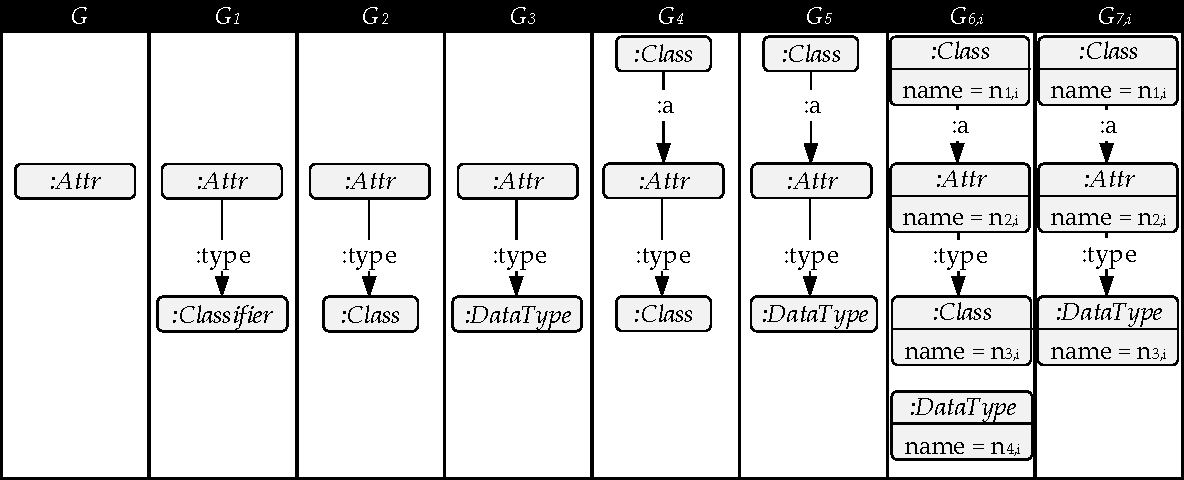
\includegraphics[width=\textwidth]{img/dc/extensions.pdf}
$Extensions(G,C)=\{\{G\},\{G_2,G_3\},\{G_4,G_3\},\{G_4,G_5\},\{G_{6,1},\ldots,G_{6,8},G_{7,1},\ldots,G_{7,5}\},\ldots\}$
\caption{$C$-extensions of Effective Atom \code{:Attr}}
\label{fig:c-extensions}
\end{figure}
\end{example}

\cref{fact:c-inc_c-ext} states that any extension of a $C$-inconsistent graph $G$ again leads to $C$-inconsistent graphs only yielding an empty extension and therefore, $C$-inconsistent graphs can be neglected in extensions.

%\nn{rename proposition to properties of C-Extensions that are demanden for the construction such that C-incosistent graphs do not need to be considered for extensions - additionally with $A=Extensions(G,C)$ with G C-inconsistent leads to $A \cup \varnothing$ AND all graphs in Extensions are not C-inconsistent except initial extension of c-inconsistent graphs - Remark 17 ins example einfuegen}

\begin{proposition}[C-Inconsistency in C-Extensions]
\label{fact:c-inc_c-ext}
Let $G$ be a graph, $C$ be a set of constraints, $E \in Extensions(G,C)$ be an extension of $G$ and $G_E \in E$ be an extended graph.
If $G_E$ is $C$-inconsistent, then $extend(G_E,\ac_P,m)=\varnothing$ for each constraint $\ac_P \equiv \vee_{i \in I} \exists (a_i\colon P \to C_i, \ac_{C_i})$ and match $m\colon P \to G_E \in \M$.
\envEndMarker
\end{proposition}

\begin{proof}
Let $G_E$ be a $C$-inconsistent graph, i.e., by \cref{def:inconsistent-graph} there exists a violation stable constraint $c \in C$ with $G_E \not\models c$.
$\M$-morphisms are closed under pushouts, i.e., $e\colon G_E \to G_E' \in \M$ in \cref{def:C-extension}, since, $f' \in \M$ and (1) is a pushout.
By \cref{def:violation-stab}, it follows that also $G_E' \not\models c$, i.e., also $G_E'$ is $C$-inconsistent.
By \cref{def:C-extension} it follows that $extend(G_E,\ac_P,m)=\varnothing$ for each constraint $\ac_P \equiv \vee_{i \in I} \exists (a_i\colon P \to C_i, \ac_{C_i})$ and match $m\colon P \to G_E \in \M$.
\end{proof}

\begin{remark}
By \cref{def:C-extension}, all graphs in $Extensions(G,C)$ are not $C$-inconsistent, except graph $G$ itself may be $C$-inconsistent as element of its initial extension $\{G\}$.
By following \cref{fact:c-inc_c-ext}, extending the initial extension for $C$-inconsistent graph $G$ via $extend(G,\_,\_)$ yields an empty extension $\varnothing \in Extensions(G,C)$.
Furthermore, contradictions in $C$ may also lead empty extensions $\varnothing \in Extensions(G,C)$, e.g., $G$ is extended via a constraint of $C$ leading to $C$-inconsistent graphs only that do not satisfy violation stable constraints of $C$.
In both cases, the existing empty extension $\varnothing$ of $G$ indicates that $G$ is not significant w.r.t. $\Lang(C)$.
\envEndMarker
\end{remark}

% \begin{remark}
% \label{rem:ext-fulfill}
% Note that for a given set of constraints $C$, only graphs are contained in
% extensions that are not $C$-inconsistent.
% This may lead to extension steps $E \Trans{extend(G_E \in E,c,\_)} E$ with
% constraint $c \in C$ that yield the same extension $E$, e.g., extension step
% $\{G_1\} \Trans{extend(G_1,c_5,\_)} \{G_1\}$ of extension $\{G_1\}$ in
% \cref{fig:c-extensions} with constraint $c_5$ in \cref{fig:constraints2}.
% Moreover, the extension step $E \Trans{extend(G_E,c,m)} E'$ that tries to
% extend a graph $G_E \in E$ via constraint $c \in C$ and match $m$ leads to an extension
% $E'= E \setminus \{G_E\}$ without $G_E$ if
% $G_E$ can not be extended at $m$ or all extensions are $C$-inconsistent. This may lead to the empty extension
% $\varnothing \in Extensions(G,C)$ for graphs $G$ that can not be embedded into
% graphs $G'$ ($G \xhookrightarrow{} G'$) such that $G' \models C$.
% \envEndMarker
% \end{remark}

% \begin{remark}
% If a constraint $\exists(P \trans{id} P, \vee_{i \in I} \exists (ac_i\colon P
% \to C_i, \true) )$ can be matched via morphism $m$ to a graph but morphisms
% $(m,ac_i)$ for some $i \in I$ are not compatible with the type inheritance, then
% the pushout (1) does not exist and we neglect the extension for the
% corresponding conclusion. If for all conclusions $ac_i$, morphisms $(m,ac_i)$
% are not compatible, then also the matched graph is neglected. Two morphisms $(m,ac_i)$
% are compatible with the type inheritance, if for all elements $e \in dom(m)=dom(ac_i)$ it holds that $m(e)$ is of the same type or a sub-type of $ac_i(e)$ or vice versa.
% \envEndMarker
% \end{remark}

For $C$-extension completeness it is sufficient to consider only the smallest graphs that occur in graphs $G \in \Lang(C)$, namely effective atoms, and from which more complex graphs can be constructed.
Atoms are the smallest graphs in the sense that they cannot be splitted into smaller sub-graphs.
With $Atoms(\ATG)$ we denote the set of atoms that are typed over an attributed type graph $\ATG$.
For (typed) attributed graphs the structure of each atom is given by either
\begin{enumerate*}[label=\itshape\alph*\upshape)]
\item an empty graph, or 
\item a single node, or 
\item a single edge together with source and target nodes, or
\item a single node attribute together with the corresponding node, or
\item a single edge attribute together with the corresponding edge and its source and target nodes.
\end{enumerate*} 
The idea of an atom $a$ is similar to the idea of an incremental monomorphism $f\colon I\rightarrowtail a$ that must exist with $I$ being the initial object (cf. \cite{DBLP:conf/wadt/CorradiniHHGN12}).
% Attributed graph morphisms $f\colon AG_1 \to AG_2$ of class
% $\mathcal{M}$ with $f=(f_G,f_D)$ are injective morphisms $f_G$ on the graph structure part and
% isomorphisms $f_D$ of algebras on the data part.
Note that all atoms in $Atoms(\ATG)$ share the same $\DSIG$-term algebra $T_\DSIG(X)$ such that the verification of domain completeness via \cref{thm:C-extensionCompleteness} is performed on the topmost level of $T_\DSIG(X)$ and therefore, can be instantiated to any concrete $\DSIG$-algebra for attributed graphs in $\Lang(C)$ and $\Lang(\GG)$ (Note that according to the general assumption, for domain completeness we assume that graphs in $\Lang(C)$ and $\Lang(\GG)$ share the same concrete $\DSIG$-algebra up to isomorphism).

\vspace{2ex}
\parpic[r][r]{
$
\SelectTips{cm}{}
     \xymatrix@R-4ex@C-4ex{
     & B \ar[dr]^{b'} & \\
     I \ar[ur]^{b} \ar[dr]_{c} & (1) & a \\
     & C \ar[ur]_{c'} & 
     }
$
}
\vspace{-2ex}
\begin{definition}[Atom]
\label{def:atom}
A \emph{graph $a$ is an atom}\index{atom}, if for each pushout (1) on the right with morphisms $b,c \in \M$ it is true that $b' \colon B \to a$ is an isomorphism or $c' \colon C \to a$ is an isomorphism.
Let $\ATG=(\TG,Z)$ be an attributed type graph with type graph $\TG$ and the final $\DSIG$-algebra $Z$ of data signature $\DSIG=(S,\OP)$ with sorts $S$ and operations $\OP$.
With $Atoms(\ATG)=\{(a=(G,T_{\DSIG}(X)),\type_G\colon a \to \ATG) \mid a \n{ is an atom},(\n{for all }e \in E^G_j\colon t^G_j(e) \in X)_{j \in \{NA,EA\}}, X=(X_s)_{s \in S} \n{ being a family of infinite sets } X_s \n{ of variables for each sort }s \in S\}$ we define the set of atoms by attributed graphs that are typed over $\ATG$ and that share the same $\DSIG$-term algebra $T_{\DSIG}(X)$ with an infinite set of variables $X_s$ for each sort $s \in S$ where each node attribute $E^G_{NA}$ and each edge attribute $E^G_{EA}$ has a variable as attribute value.
\envEndMarker
\end{definition}

Given a set of constraints $C$ that are typed over attributed type graph $\ATG$, then with $EAtoms(C)$ we denote the set of effective atoms w.r.t. language $\Lang(C)$.
Effective atoms are those atoms in $Atoms(\ATG)$ that occur in graphs $G \in \Lang(C)$.

\begin{definition}[Effective Atom]
\label{def:eatom}
Given language $\Lang(C)$ over attributed type graph $\ATG$ and constraints $C$, an \emph{atom $a \in Atoms(ATG)$ is effective w.r.t. $\Lang(C)$}\index{atom!effective}, if there exists an inclusion $i\colon a \to G \in \M$ for some graph $G \in \Lang(C)$.
With $EAtoms(C)=\{a \mid a \in Atoms(\ATG), a \n{ is effective w.r.t. }\Lang(C)\}$ we denote the set of effective atoms w.r.t. $\Lang(C)$.
\envEndMarker
\end{definition}

\begin{example}[Effective Atom]
Given the constraints $C$ for UML class diagrams in \cref{sec-gt-gc,ex:sec-gc-gc:gc_UML_CD}, then the effective atoms w.r.t. $\Lang(C)$ are those atoms in $Atoms(\TG_{\CD})$ that fulfill the domain constraints for abstract types from \cref{ex:sec-gc-gc:gc_UML_CD}.
Graphs $G,G_2$ and $G_3$ in \cref{fig:c-extensions} are effective atoms w.r.t. $\Lang(C)$.
Graph $G_1$ is an atom but not effective, since, \code{Classifier} is an abstract type and therefore, $G_1$ violates the constraints for abstract types.
Graphs $G_4$ to $G_{7,5}$ are not atoms.
\envEndMarker
\end{example}

For $C$-extension completeness, in practice we consider atoms up to isomorphism only.
Given a set of constraints $C$ that are typed over type graph $\ATG$, then $C$-extension completeness of a given language $\Lang$ over $\ATG$ states that for all effective atoms w.r.t. $\Lang(C)$ that are typed over $\ATG$, an extension via constraints $C$ can be found that is in $\Lang$.

\begin{definition}[$C$-Extension Completeness]
\label{def:C-extensionCompleteness}
Let $C$ be a set of constraints typed over $\ATG$ and $C' \subseteq C$ be the contained constraints that are designated for general satisfaction.
Then, a language $\Lang$ over $\ATG$ is called \emph{$C$-extension complete}\index{$C$-extension completeness}, if $\forall a \in EAtoms(C). \exists S \in Extensions(a, C')$ such that $S \subseteq \Lang$.
\envEndMarker
\end{definition}

\begin{example}[$C$-Extension Completeness]
\label{ex:c-extension-compl}
\begin{figure}[tb]
\centering
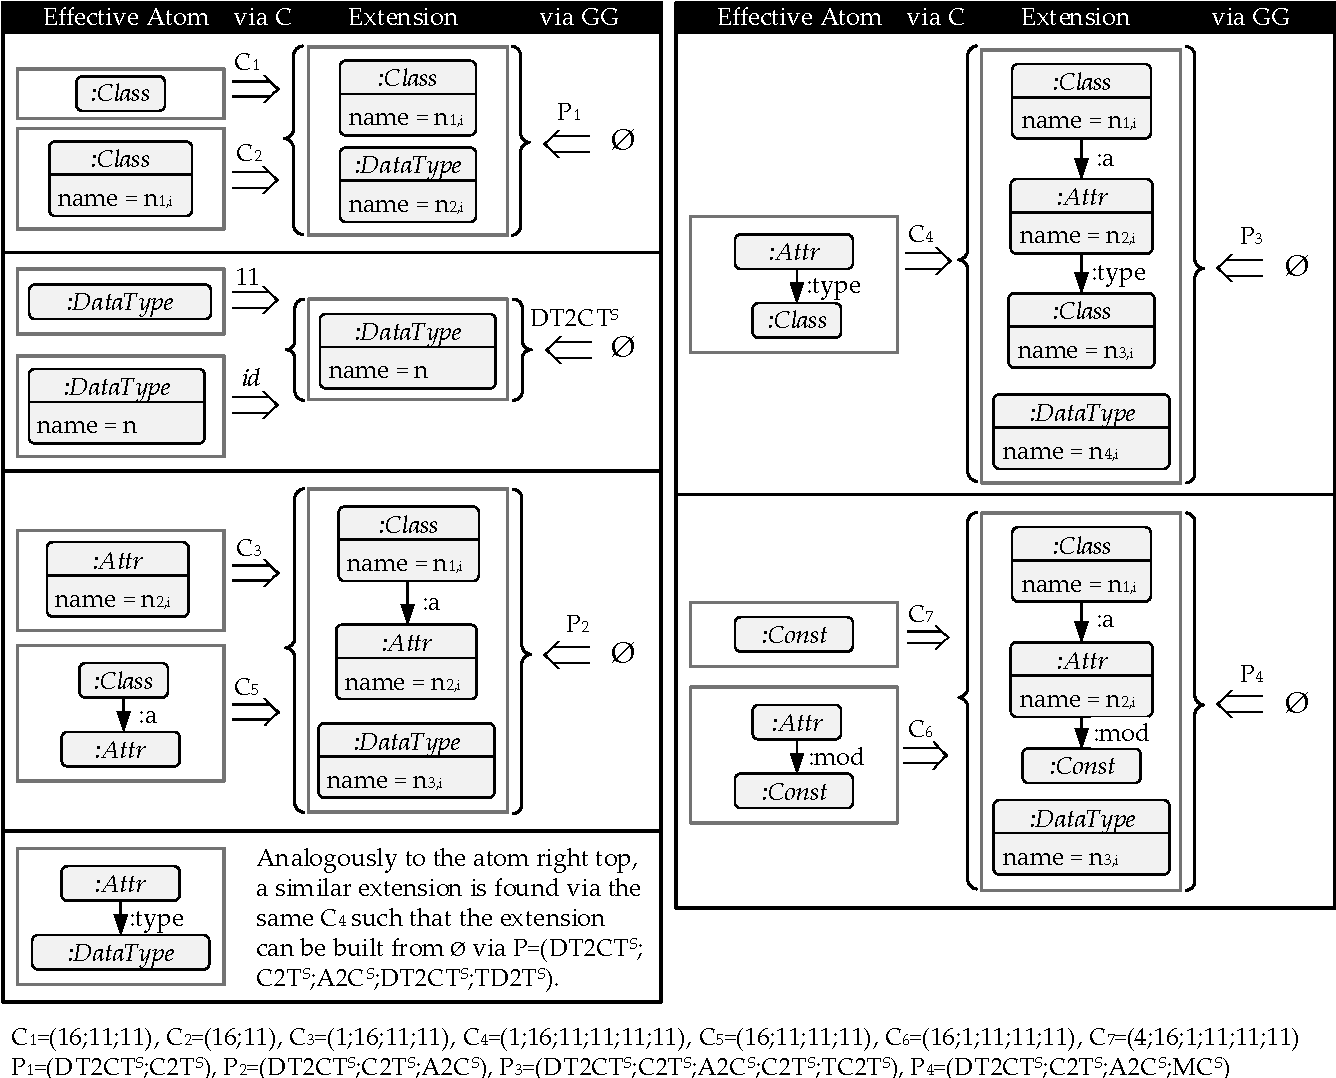
\includegraphics[width=\textwidth]{img/dc/example_compl}
\caption{Verifying $C$-Extension Completeness of Language $\Lang(\GG)$ for UML Class Diagrams}
\label{fig:eatoms_check}
\end{figure}
Given the rules $P$ for creating UML class diagrams from \cref{sec-gt-trafo,ex:sec-gt-trafo:trafo} together with grammar $\GG=(\varnothing,P)$ that is typed over $\TG_\CD$ in \cref{sec-gt-graphs,fig:sec-gt-graphs:atg} and the constraints $C$ for class diagrams typed over $\TG_\CD$ from \cref{sec-gt-gc,ex:sec-gc-gc:gc_UML_CD}.
We show $C$-extension completeness of language $\Lang(\GG)$ over $\TG_\CD$. 
For each effective atom in $EAtoms(C)$ an extension via constraints $C$ must be constructed that is a subset of language $\Lang(\GG)$.
Similarly to \cref{ex:c-extensions}, we write the actual constraints but mean their instances according to \cref{def:C-extension} and furthermore, each graph with attribute values $n_{1,i}$ to $n_{4,i}$ in \cref{fig:eatoms_check} represents a set of graphs that contains all combinations of equal and unequal values $n_{1,i}$ to $n_{4,i}$ except equal values for $n_{1,i}$ and $n_{3,i}$ if both represent the \code{name}s of distinct \code{Class}es.
An extension is a subset of $\Lang(\GG)$, if all graphs of the extension can be constructed via rules $P$ from start graph $\varnothing$ of $\GG$.
The effective atoms $EAtoms(C)$ are given by graph $G$ in \cref{fig:c-extensions} together with the effective atoms in \cref{fig:eatoms_check}.
For atom $G$, extension $\{G_{6,1},\ldots,G_{6,8},G_{7,1},\ldots,G_{7,5}\} \in Extensions(G,C)$ can be constructed by extending $G$ via constraints $(8;1;1;11;11;11;16;11;11;11;11)$ of $C$ successively (cf. \cref{ex:c-extensions}).
Each graph of the extension can be constructed by applying rules \code{(DT2CT^S;C2T^S;A2C^S;C2T^S;TC2T^S)} or \code{(DT2CT^S;C2T^S;A2C^S;TD2T^S)} successively with starting at the empty start graph $\varnothing$ of $\GG$.
All other effective atoms are also successfully checked as depicted in \cref{fig:eatoms_check}.
Therefore, language $\Lang(\GG)$ is $C$-extension complete.
% \begin{itemize}
%   \item Atom \xymatrix{*+[F]\txt{:Class}} can be extended with constraints $c_8$
%   to extension $\left\{\xymatrix{*+[F]\txt{:Class(name=n)}}\right\}$ which can be
%   constructed by source rule \code{1:~C2T$_S$}.
%   \item Atom \xymatrix{*+[F]\txt{:Class(name=n)}} can be directly constructed by
%   source rule \code{1:~C2T$_S$}.
%   \item Atom \xymatrix{*+[F]\txt{:PrimitiveType}} can be extended with
%   constraint $c_8$ to extension
%   $\left\{\xymatrix{*+[F]\txt{:PrimitiveType(name=n)}}\right\}$ which can be constructed by
%   source rule \code{2:~PT2CT$_S$}
%   \item Atom \xymatrix{*+[F]\txt{:PrimitiveType(name=n)}} can be
%   directly constructed by source rule \code{2:~PT2CT$_S$}
%   \item Atom \xymatrix{*+[F]\txt{:Attribute(name=n)}} is checked analogously to \cref{ex:c-extension-compl} but this time the extensions for the \code{name} attribute are omitted.
%   \item Atom \xymatrix{*+[F]\txt{:Attribute(is\_primary=true)}} can be extended with constraints in the given order $(c_{10},c_1,c_8^*)$ leading to extension \begin{align*}
%   \left\{\xymatrix{*+[F]\txt{:Class\\(name=n1)} \ar[r]^-{:attrs} & *+[F]\txt{:Attribute\\(is\_primary=true,\\name=n2)} \ar[r]^-{:type} & *+[F]\txt{:PrimitiveType\\(name=n3)}} \right\}
%   \end{align*} which can be constructed by applying the following source rules in the given order: (\code{1:~C2T$_S$}, \code{2:~PT2CT$_S$}, \code{3:~PA2C$_S$}, \code{4:~AM2CM$_S$}, \code{5:~P2PK$_S$}).
%   \item Atom \xymatrix{*+[F]\txt{:Attribute(is\_primary=false)}} can be extended with constraints in the given order $(c_5,c_4,c_8^*)$ leading to an extension with two graphs \begin{align}
%   G_1=\xymatrix{*+[F]\txt{:Attribute\\(is\_primary=false,\\name=n1)} \ar[r]^-{:type} & *+[F]\txt{:PrimitiveType\\(name=n2)}}\\
%   G_2=\xymatrix{*+[F]\txt{:Attribute\\(is\_primary=false,\\name=n1)} \ar[r]^-{:type} & *+[F]\txt{:Class\\(name=n2)}}
%   \end{align} which can be constructed by applying the following source rules in the given order: (\code{2:~PT2CT$_S$}, \code{3:~PA2C$_S$}, \code{7:~NP2E$_S$}) for $G_1$ and (\code{1:~C2T$_S$}, \code{6:~NPA2C$_S$}, \code{7:~NP2E$_S$}) for $G_2$.
%   \item Analogously, atoms \xymatrix{*+[F]\txt{:Class} \ar[r]^-{:attrs}& *+[F]\txt{:Attribute}}, \xymatrix{*+[F]\txt{:Attribute} \ar[r]^-{:type}& *+[F]\txt{:Class}} and \xymatrix{*+[F]\txt{:Attribute} \ar[r]^-{:type}& *+[F]\txt{:PrimitiveType}} can be checked.
% \end{itemize}
\envEndMarker
\end{example}

% \begin{remark}
% In the
% presented setting, only language inclusions $\Lang_1=\Lang(\ATG,C) \subseteq
% \Lang_2=\Lang(\ATG,\GG,C)$ between languages with the same set of constraints
% $C$ are considered. Therefore, we are only interested in the C-extension completeness
% of languages $\Lang_2$ where $\Lang_2$ is restricted
% by $C$. Consequently, for efficiency reasons the derivation and checking of
% extensions can be stopped at extensions that violate negative constraints in $C$, since,
% these extensions and all other derivations of such extensions are not in
% $\Lang_2$.
% \envEndMarker
% \end{remark}

%A union $A +_I B$ of two objects $A$ and $B$ is 
%constructed by finding an intersection $I$ with embeddings (\M-morphisms)
%$a \colon I \to A, b\colon I\to B$ and constructing the pushout of $a$ and $b$ 
%yielding the pushout object $C = A +_I B$.

%\begin{definition}[Closure under Union]
%\label{def:closedness-union}
%A language $\Lang$ is closed under union, if any union $A +_I B$ of two elements $A,B \in \Lang$
%is contained in $\Lang$.
%\envEndMarker
%\end{definition}

%\begin{lemma}[C-Extension Completeness and closure]
%\label{lem:C-extension-closure}
%Let $C$ be a set of constraints typed over $TG$ and 
%$\Lang$ be a $C$-extension complete language that is closed under union.
%Then, $\Lang(TG,C) \subseteq \Lang$.
%\envEndMarker
%\end{lemma}
%
%\begin{proof}
%to be done - Benjamin/Nico??
%\end{proof}

% \longversionMarker{
% \begin{remark}
% Note that the problem of whether a language is C-extension completeness is only
% semi-decidable but not decidable in general. If a language
% $\Lang$ is C-extension complete, then for each effective atom
% an extension can be found that is in $\Lang$ but for languages that are not
% C-extension complete we may not neglect this fact. Note that for the generation
% of extensions, for each constraint and match only one instance of the constraint
% must be considered which is obtained by the $\E$--$\M$-factorization of the
% match morphism (cf.\cref{cor:AC-schemata-satisfaction}).
% In practice, the size of the graphs in $\Lang$ is limited to a maximal number \emph{MAX} of graph elements in order to obtain decidability of the problem. This reduces the verification to extensions up to a size of \emph{MAX} graph elements.
% \envEndMarker
% \end{remark}
% }

In addition to $C$-extension completeness another property called $C$-conflict-freeness of marking rules is neccessary in order to verify full language inclusions $\Lang(C) \subseteq \Lang(\GG)$ of domain completeness.
Based on the notions of translation attributes in \cref{sec-mt-tgg,rem:sec-mt-tgg:tr_attr} and consistency creating (CC) rules in \cref{sec-msynch-tgg,def:sec-msynch-tgg:cc_rule}, we define marking rules for non-deleting flat grammars with application conditions in \cref{def:marking-rule}.
In the context of marking rules, we take marking attribute as synonym for translation attribute.
For a non-deleting grammar $\GG$, the set of marking rules $m(\GG)$ contains for each rule $r \in \GG$, a marking rule $m(r)$.
Analogously to CC rules, marking rules are derived from rules by adding marking attributes with value $\False$ (false) or $\True$ (true) to all elements (nodes, edges or attributes) of the rule.
Whenever rule $r$ creates an element, then marking rule $m(r)$ preserves this element and updates its marking attribute from $\False$ to $\True$, denoted by $[\False => \True]$.
Whenever rule $r$ preserves an element, then marking rule $m(r)$ also preserves this element and leaves its marking attribute set to $\True$.
Thus, marking rules are deleting on the marking attributes and allow a conflict analysis of (common) created elements which cannot be performed directly on the non-deleting rules themselves.
Furthermore, all elements of the application condition of rule $r$ that are not contained in the left-hand side of the rule need to be extended by a marking attribute with value $\True$.
Therefore, we use the concept of $\True$-extended application conditions from \cref{sec-mt-tgg,def:sec-mt-tgg:T-Ext} and restrict it from triple graphs to flat graphs by omitting the triple components $X$.

% \begin{remark}[Well-Definedness of $\True$-Extension]
% Note that $P' +_P C$ denotes the gluing of graphs $P'$ and $C$ over shared graph $P$ (constructed as a pushout).
% The $\True$-Extension construction is well-defined in the category $\AGraphs_{\ATGI}$, as, morphism $P \to P'$ is an identity on the data part by construction of graphs with marking attributes (i.e., $a_D$ can be used for $a_E$) and $\AGraphs_{\ATGI}$ is $\M$-adhesive (i.e., pushouts exist along $\M$-morphisms and $\M$-morphisms are closed under pushouts, thus, $\inc'_P$ is an inclusion). 
% \envEndMarker
% \end{remark}

\begin{definition}[Marking Rule]
\label{def:marking-rule}
Given a non-deleting rule $p=\nobreak(\ol{p}\colon L \xhookrightarrow{} R,\ac_L)$, the \emph{marking rule $m(p)=(L_M \xhookleftarrow{l_M} K_M \xhookrightarrow{r_M} R_M,\ac_{L_M})$ of $p$}\index{marking rule} is constructed component-wise for $L_M,K_M,R_M$ and $\ac_{L_M}$ with induced inclusions $l_M,r_M$ and $L_M := R \oplus \Att_{\ol{p}(L)}^{\True} \oplus \Att_{R\setminus \ol{p}(L)}^{\False}, K_M := R \oplus \Att_{\ol{p}(L)}^{\True}, R_M := R \oplus \Att_R^{\True}$ and $\ac_{L_M}=\tExt(\ac_L,L_M)$.
Let $\GG=(S,P)$ be a non-deleting graph grammar.
With $m(\GG)=\{m(p) \mid p \in P\}$ we define the set of marking rules for all rules in $\GG$.
\envEndMarker
\end{definition}

\begin{remark}[Termination of Transformation System $m(\GG)$]
\label{rem:sec-dc-verification:term_marking_rules}
Although marking rules are not directly applied for verifying domain completeness, we state the following interesting property:
If all rules $p=(L \xhookrightarrow{} R,\ac_L)$ of a non-deleting grammar $\GG$ are non-trivial in the sense that $L$ and $R$ are not isomorphic ($L \not\cong R$) and therefore, each rule creates at least one element, then the transformation system $m(\GG)$ of marking rules is terminating for finite graphs, since, each application of marking rules updates the marking attributes of at least one graph element from $\False$ to $\True$ as long as all graph elements are marked with $\True$ or no marking rule is applicable anymore.
\envEndMarker
\end{remark}

\begin{example}[Marking Rule]
\label{ex:sec-dc-verification:marking_rule}
\begin{figure}[tb]
\centering
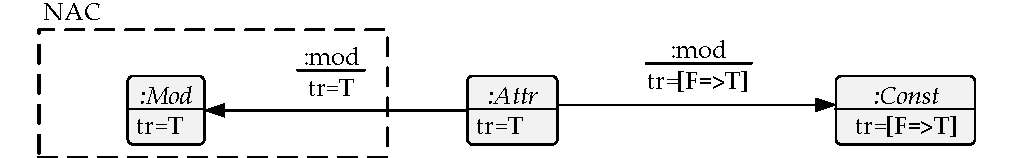
\includegraphics[width=.9\textwidth]{img/dc/markingrule-VOLT.pdf}
\caption{Marking Rule $m(\code{4}^S)$ of Rule $\code{4}^S$ for UML Class Diagrams}
\label{fig:sec-dc-verification:marking_rule}
\end{figure}
The marking rule $m(\code{4}^S)$ of source rule $\code{4}^S$ from \cref{sec-gt-trafo,ex:sec-gt-trafo:trafo} is given by the rule in \cref{fig:sec-dc-verification:marking_rule}.
Marking attributes $\tr$ are added to all elements and they are updated from $\False$ to $\True$ ($[\False => \True]$) for those elements that are created by rule $\code{4}^S$ while the marking attributes of all other elements are initially set to $\True$ and remain unchanged.
\envEndMarker
\end{example}

The $C$-conflict-freeness of marking rules is checked based on critical pair analysis.
According to \cref{def:consistent-critical-pair} and similarly to $C$-inconsistent graphs, a critical pair $(K_1 \TransB{} O \Trans{} K_2)$ is $C$-inconsistent if graph $O$ does not satisfy a constraint in $C$ that is violation stable under embedding.
$C$-inconsistent critical pairs do not need to be analysed for verifying domain completeness, since, such critical pairs and any of their embeddings into larger contexts do not occur in graphs $G \in \Lang(C)$.
The marking rules are $C$-conflict-free, if for each critical pair $(K_1 \TransB{(p_1,o_1)}\nobreak O \Trans{(p_2,o_2)} K_2)$ that is not $C$-inconsistent with marking rules $p_1$ and $p_2$, the rules and matches are the same $(p_1=p_2,o_1=o_2)$ (cf. \cref{def:cf-marking-rules}).

\begin{definition}[$C$-Inconsistent Critical Pair]
\label{def:consistent-critical-pair}
Let $C$ be a set of constraints. 
A \emph{critical pair $(K_1 \TransB{} O \Trans{} K_2)$ is $C$-inconsistent}\index{critical pair!$C$-inconsistent}, if conflict graph $O$ is $C$-inconsistent. 
\envEndMarker
\end{definition}

\parpic[r][r]{
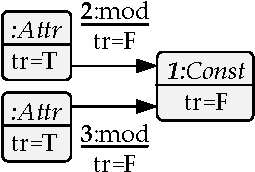
\includegraphics[width=.23\textwidth]{img/dc/c_inc_cp.pdf}
}
\vspace*{-.25cm}
\begin{example}[$C$-Inconsistent Critical Pair]
\label{ex:c_inc_cp}
The figure on the right presents the conflict graph $O$ of the critical pair $(K_1 \TransB{(m(4^S),m_1)} O \Trans{(m(4^S),m_2)} K_2)$ with marking rule $m(4^S)$ from \cref{ex:sec-dc-verification:marking_rule}.
Transformation $O \Trans{(m(4^S),m_1)} K_1$ updates the marking attributes of node \code{1:Const} and edge \code{2:mod} and $O \Trans{(m(4^S),m_2)} K_2$ updates the marking attributes of \code{1:Const} and edge \code{3:mod} from $\False$ to $\True$.
This corresponds to a delete-use conflict at node \code{1:Const} in $O$, since, both transformations change its marking attribute where the attribute is deleted at first and added with the new value $\True$ afterwards.
However, by assuming the constraints $C$ for UML class diagrams from \cref{sec-gt-gc,ex:sec-gc-gc:gc_UML_CD}, the critical pair is $C$-inconsistent, since, $O \not\models 7$ and constraint $7 \in C$ is violation stable under embedding, i.e., graph $O$ is $C$-inconsistent (cf. \cref{ex:constraints-violation-stable}).
\envEndMarker
\end{example}

Analogously, to significant graphs, we introduce significant critical pairs.
A critical pair is significant, if it occurs in graphs $G \in \Lang(C)$.
Also analogously to significant and $C$-inconsistent graphs, $C$-inconsistent critical pairs are only a subset of not significant critical pairs but can be identified more efficiently.

% Significant critical marking pairs describe pairs $P_1 \TransB{(m(p_1),m_1)} K \Trans{(m(p_2),m_2)} P_2$ of transformations via marking rules $m(p_1),m(p_2)$ where the sub-graph $K'$ of $K$ marked with $\True$ can be created via $P$ (possibly in bigger contexts $K''$) and $K'$ ($K''$) is contained in graphs of $\Lang(\TG,C)$ (and creating rules $p_1,p_2 \in P$ are applicable to $K''$ with matches compatible to inclusion $K' \xhookrightarrow{} K''$).
% Thus, we only consider parallel dependent transformation steps that may occur when creating graphs of $\Lang(\TG,C)$ via $P$.
\begin{definition}[Significant Critical Pair]
\label{def:sig_crit_pair}
Let $C$ be a set of constraints, $\GG$ be a non-deleting grammar and $m(\GG)$ be the corresponding set of marking rules.
A \emph{critical pair $(K_1 \TransB{(p_1,m_1)} O \Trans{(p_2,m_2)} K_2)$ for marking rules $p_1,p_2 \in m(\GG)$ is significant w.r.t. $\Lang(C)$}\index{critical pair!significant}, if conflict graph $O$ is significant w.r.t. $\Lang(C)$.
\envEndMarker
\end{definition}

\begin{remark}[Relationship between $C$-Inconsistent \& Significant Critical Pairs]
\label{rem:sec-dc-verification:rel_critical_pair}
Similarly to the relationship between $C$-inconsistent and significant graphs in \cref{rem:sec-gc-verification}, by definition, each $C$-inconsistent critical pair is not significant w.r.t. $\Lang(C)$.
Furthermore, each critical pair that is significant w.r.t. $\Lang(C)$ is not $C$-inconsistent.
The other directions do not hold in general.
\envEndMarker
\end{remark}

\begin{figure}[tb]
\centering
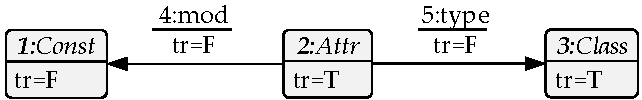
\includegraphics[width=.65\textwidth]{img/dc/sign_cp.pdf}
\caption{Significant Critical Pair}
\label{fig:sec-dc-verification:sign_critical_pair}
\end{figure}

\begin{example}[Significant Critical Pair]
\label{ex:sign_cp}
The graph in \cref{fig:sec-dc-verification:sign_critical_pair} presents the conflict graph $O$ of the critical pair $(K_1 \TransB{(m(4^S),m_1)} O \Trans{(m(6^S),m_2)} K_2)$ with marking rules $m(4^S)$ and $m(6^S)$ of the rules in \cref{sec-gt-trafo,ex:sec-gt-trafo:trafo}.
Transformation $O \Trans{(m(4^S),m_1)} K_1$ updates the marking attributes of edge \code{4:mod} and node \code{1:Const} from $\False$ to $\True$ leading to a graph pattern which is forbidden by the NAC of rule $m(6^S)$ with match $m_2$ (change-forbid attribute conflict).
Given the constraints $C$ for UML class diagrams from \cref{sec-gt-gc,ex:sec-gc-gc:gc_UML_CD}, then the critical pair is not $C$-inconsistent, since, $O$ does not violate a constraint $c \in C$ which is violation stable under embedding.
However, the critical pair is not significant, since, graph $O$ is not significant w.r.t. $\Lang(C)$ (cf. \cref{ex:sec-dc-verification:inc_sig_graph}).
\envEndMarker
\end{example}

% \begin{lemma}[C-Extension Completeness for Conflict-free Grammar]
% \label{lem:conflictFree}
% Let $C$ be a set of constraints $C$ and
%  $\GG$ be a graph grammar. 
% If all marking rules $p \in m(GG)$ are $C$-conflict-free
% and $\Lang(GG)$ is $C$-extension complete, then 
% $\Lang(TG,C) \subseteq \Lang(GG)$.
% \envEndMarker
% \end{lemma}

%\begin{corollary}[Closure for Conflict-free Grammar]
%\label{cor:conflictFree-closure}
%Let $\GG$ be a non-deleting graph grammar
%and $C$ be a set of constraints, such that 
%$\Lang(\GG,C) = \Lang(\GG)$.
%If for each critical pair of
%$m(\GG)$ that is not C-inconsistent the rules and matches are the same and $m(\GG)$ is
%terminating, then $\Lang(GG,C)$ is closed under union.
%\envEndMarker
%\end{corollary}
%
%\begin{proof}
%to be done using \cref{lem:conflictFree-closure}.
%\end{proof}





% \begin{definition}[Graph with marking attributes]
% An attributed graph $\AG=(G,D)$ is a graph with marking attributes, if $G$ is
% extended by one boolean marking attribute for each element in $G$ (node or edge)
% and by one boolean marking attribute for each attribute of an element with
% $ATT_G$ being the extension of $G$. $ATT_G^v$ with $v=\True$ or $v=\False$ denotes a
% graph where all marking attributes are set to true or false. With $AG \oplus
% ATT_{G_0}^v$ and $G_0 \subseteq G$ we denote an attributed graph AG where all
% attributes of the subgraph $G_0$ are set to true or false.
% \end{definition}

\begin{figure}[tb]
\centering
% 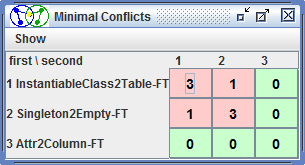
\includegraphics[width=.55\textwidth]{figs/agg.png}
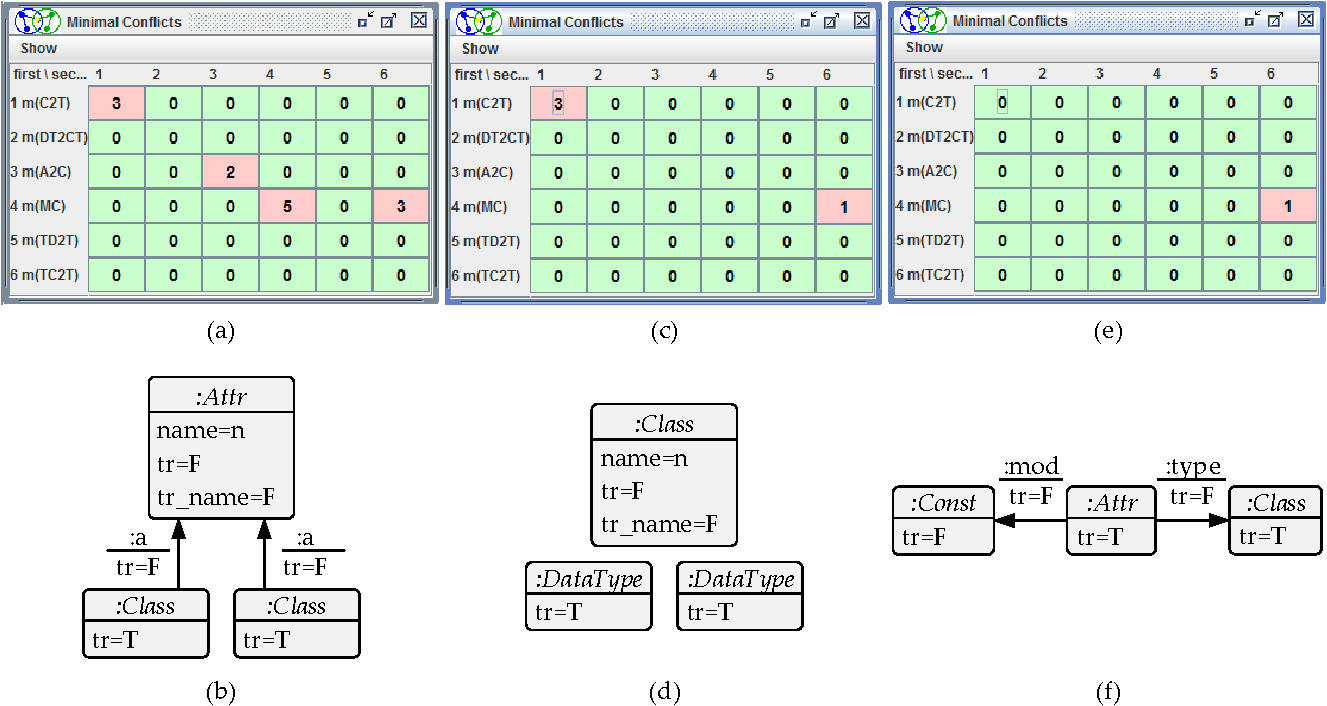
\includegraphics[width=\textwidth]{img/dc/agg.pdf}
\caption{Result of Conflict Analysis for Marking Rules of UML Class Diagrams in AGG}
\label{fig:agg}
\end{figure}

\begin{definition}[$C$-Conflict-Freeness of Marking Rules]
\label{def:cf-marking-rules}
Let $C$ be a set of constraints and let $m(\GG)$ be the marking rules of a non-deleting grammar $\GG$.
Then, \emph{$m(\GG)$ is $C$-conflict-free}\index{marking rule!$C$-conflict-freeness}, if for each critical pair $(K_1 \TransB{(p_1,o_1)}\nobreak O \Trans{(p_2,o_2)} K_2)$ that is significant w.r.t. $\Lang(C)$ (or not $C$-inconsistent) with $p_1,p_2 \in m(\GG)$ it is true that the rules and matches are the same ($p_1=p_2,o_1=o_2$) (or it is true that the critical pair is strictly confluent).
\envEndMarker
\end{definition}

\begin{remark}[$C$-Conflict-Freeness of Marking Rules]
\label{rem:sec-dc-verification:conf_free_mr}
The critical pairs in \cref{def:cf-marking-rules} need to be significant or not $C$-inconsistent.
Analogously to \cref{rem:sec_dc-verification:c-ext}, claiming that the critical pairs are significant is more accurate for verifying domain completeness based on $C$-conflict-freeness of marking rules in \cref{def:cf-marking-rules,thm:C-extensionCompleteness}, since, critical pairs may be not $C$-inconsistent and not significant at the same time (cf. \cref{ex:sign_cp}).
While not $C$-inconsistent critical pairs are considered in $C$-conflict-freeness of marking rules, not significant critical pairs are not considered.
However, claiming that the critical pairs are not $C$-inconsistent can be checked more efficiently.
Furthermore, claiming that each critical pair is strictly confluent is a stronger condition and harder to check than claiming that each critical pair is of same rules and same matches.
Each critical pair of same rules and same matches is directly strict confluent by definition.
\envEndMarker
\end{remark}

\begin{example}[$C$-Conflict-Freeness of Marking Rules]
\label{ex:conflict-freeness-marking-rules}
The AGG-tool \cite{AGG} is used to help verifying $C$-conflict-freeness of marking rules $m(\GG)$ for grammar $\GG=(S,P)$ with rules $P$ for UML class diagrams from \cref{sec-gt-trafo,ex:sec-gt-trafo:trafo} and constraints $C$ for UML class diagrams from \cref{sec-gt-gc,ex:sec-gc-gc:gc_UML_CD}.
AGG enables to analise conflicts of rules, outputs all existing critical pairs and allows to ignore
\begin{enumerate*}
\item critical pairs of same rules and same matches,
\item critical pairs that violate multiplicity constraints, and
\item critical pairs that are directly strict confluent.
\end{enumerate*}
\cref{fig:agg} depicts the result of the analysis for the marking rules $m(\GG)$ of UML class diagrams.
\cref{fig:agg} (a) depicts all 13 critical pairs of marking rules $m(\GG)$ (red boxes) while ignoring all critical pairs of same rules and same matches.
\cref{fig:agg} (b) depicts the conflict graph of the critical pair of rule $\code{3}^S$ that updates the marking attributes of node \code{:Attr} and edges \code{:a} in parallel while matching differently to both \code{:Class} nodes.
The conflict graph violates multiplicity constraint \code{2} which is violation stable under embedding (cf. \cref{ex:constraints-violation-stable}).
Therefore the conflict graph is $C$-inconsistent implying further that the critical pair is $C$-inconsistent.
\cref{fig:agg} (c) depicts all four critical pairs of marking rules $m(\GG)$ while additionally ignoring all critical pairs that violate the multiplicity constraints in $C$.
\cref{fig:agg} (d) depicts the conflict graph of the critical pair of rule $\code{1}^S$ that updates the marking attributes of node \code{:Class} in parallel while matching differently to both \code{:DataType} nodes.
The conflict graph is not $C$-inconsistent, particularly it respects the multiplicity constraints.
However, the conflict graph is directly strict confluent, i.e., the critical pair is directly strict confluent.
\cref{fig:agg} (e) depicts the only critical pair of marking rules $m(\GG)$ while additionally ignoring all critical pairs that are directly strict confluent.
\cref{fig:agg} (f) depicts the conflict graph of the critical pair of rules $\code{4}^S$ and $\code{6}^S$ that updates the marking attributes of node \code{:Const} and edges \code{:mod}, \code{:type} in parallel while matching node \code{:Attr} in common.
The critical pair is not strictly confluent due to the NAC of rule $\code{6}^S$.
Furthermore, the critical pair is not $C$-inconsistent, particularly it does not violate the multiplicity constraints in $C$.
However, the critical pair is not significant (cf. \cref{ex:sign_cp}).
Therefore, the marking rules $m(\GG)$ of UML class diagrams are $C$-conflict-free.
\envEndMarker
\end{example}

% \begin{fact}[Characterisation of Grammars with C-conflict-free Marking Rules]
% Let $GG=(\ATG,\SG,P)$ be a grammer with non-deleting rules $P$ typed over
% $\ATG$ and let $C=C^{IN} \cup C^{OUT} \cup C^{Att}$ be a set of
% multiplicity constraints. The constraints in $C^{IN(OUT)}$ claim for a set of
% edge types $E(C^{IN(OUT)})$ that for all types $t \in E(C^{IN(OUT)})$, each node
% may have at most one incoming (outgoing) edge of type $t$. The
% constraints in $C^{Att}$ claim for a set of attributes $Att(C^{Att})$ that
% for all attributes $a \in Att(C^{Att})$, each node may have at most one
% attribute $a$.The marking rules $m(\GG)$ are C-conflict free iff for each rule
% $p \in P$:
% \begin{itemize}
%   \item $p$ creates at most one node of each type, and no other rule $p'
%   \in P$ creates nodes of the same types, or
%   \item 
% \end{itemize}
% \envEndMarker
% \end{fact} 

The main result for verifying domain completeness is stated by \cref{thm:C-extensionCompleteness}.
Intuitively, the language inclusion $\Lang(C) \subseteq \Lang(\GG)$ holds if each graph $G \in \Lang(C)$ can be decomposed into its atoms $a \subseteq G$ such that for each atom $a$ an extension $E$ can be constructed via constraints $C$ that is contained in $\Lang(\GG)$ and the composition of the extensions leads to graph $G$ in $\Lang(\GG)$ again by applying the rules of grammar $\GG$.
The verification approach requires that all productions of grammar $\GG$ are non-trivial.
For non-trivial productions we refer to \cref{rem:sec-dc-verification:term_marking_rules}.

\begin{theorem}[Domain Completeness]
\label{thm:C-extensionCompleteness}
\index{domain completeness!verification}
Let $\Lang(C)$ be a language over type graph $\ATG$ and constraints $C$ in $\M$-normal form and let $\Lang(\GG)$ be a language over $\ATG$ and non-deleting grammar $\GG=(\varnothing,P)$ with empty start graph $\varnothing$, all productions $p \in P$ being non-trivial and where all application conditions in productions $P$ are in $\M$-normal form.
If the marking rules $m(\GG')$ are $C$-conflict-free and $\Lang(\GG')$ is $C$-extension complete where $\GG'=(\varnothing',P)$ with $\varnothing'$ being the empty start graph with $\DSIG$-term algebra $T_\DSIG(X)$, then domain completeness holds for almost injective matches $m \in \morO$, i.e., it holds that $\Lang(C) \subseteq \Lang(\GG)$.
\envEndMarker
\end{theorem}

\begin{proof}[Idea]
Let $G \in \Lang(C)$.
Graph $G$ is abstracted to a graph $G_A$ with $\DSIG$-term algebra.
$G_A$ can be decomposed into its atoms $Atoms(G_A)$ by \cref{lemma:union-atoms}.
$C$-extension completeness of $\Lang(\GG')$ ensures that each atom can be extended via $C$ such that the extension can be created via grammar $\GG'$.
Furthermore, there is a gluing of all extensions leading to graph $G_A$ again by \cref{lem:union-ext-atoms}.
By the equivalence of marking and transformation sequences in \cref{lem:equivalence-marking-emptySG}, each extension can be fully marked with $\True$.
The $C$-conflict freeness of the marking rules $m(\GG')$ allows to apply confluence results and we derive a marking sequence that fully marks $G_A$. 
Thus by \cref{lem:equivalence-marking-emptySG}, there is a transformation sequence $\varnothing' \Trans{*} G_A$ via $P$.
By \cref{lem:atiti}, there is a transformation $\varnothing \Trans{*} G$ via $P$, i.e., $G \in \Lang(\GG)$.
The full proof is presented in \cref{sec-proofs:thm:C-extensionCompleteness}.
\end{proof}

We successfully verified domain completeness $\Lang(C) \subseteq \Lang(\GG)$ for constraints $C$ of UML class diagrams from \cref{sec-gt-gc,ex:sec-gc-gc:gc_UML_CD} and grammar $\GG=(\varnothing,P)$ with rules $P$ for UML class diagrams from \cref{sec-gt-trafo,ex:sec-gt-trafo:trafo}.
$C$-extension completeness of language $\Lang(\GG)$ is successfully verified in \cref{ex:c-extension-compl}.
$C$-conflict-freeness of the marking rules $m(\GG)$ is successfully verified in \cref{ex:conflict-freeness-marking-rules} by claiming that the critical pairs are significant and strictly confluent (cf. \cref{rem:sec-dc-verification:conf_free_mr}).
Therefore, all graphs $G \in \Lang(C)$ can be constructed via grammar $\GG$.
This means that the domain constraints $C$ are strict enough to cover all language restrictions that are induced by grammar $\GG$.
Note that if $C$-extension completeness of $\Lang(\GG)$ or $C$-conflict-freeness of marking rules $m(\GG)$ does not hold, then their verification may lead to minimal examples of graphs $G \in \Lang(C)$ that cannot be constructed via grammar $\GG$.
Such examples may serve as helpful hints for refactoring the grammar or determining which constraints need to be added to or removed from $C$ in order to obtain domain completeness ($\Lang(C) \subseteq \Lang(\GG)$).

In order to ensure termination for the verification of domain completeness via \cref{thm:C-extensionCompleteness}, one can define a finite upper bound $G_u$ for the size of graphs $G \in \Lang(C)$, i.e., only graphs $G \in \Lang(C)$ with inclusions $G \to G_u \in \M$ are considered (cf. \cref{def:sec-dc-verification:dc_ub}).
In most cases, the verification terminates without restricting to an upper bound as shown in \cref{ex:c-extension-compl,ex:conflict-freeness-marking-rules}.
Note that by restricting to an upper bound we could also check for all graphs up to the upper bound which satisfy the constraints in $C$ if they can be created via the rules in grammar $\GG$ for ensuring the validity of language inclusion $\Lang(C) \subseteq \Lang(\GG)$ up to the upper bound.
However, the verification via $C$-extension completeness in \cref{thm:C-extensionCompleteness} is more efficient in most cases, since, not all graphs need to be checked but rather a small subset.

\begin{definition}[Domain Completeness up to Upper Bound]
\label{def:sec-dc-verification:dc_ub}
\index{domain completeness!up to upper bound}
Given the context of domain completeness in \cref{sec-dc-general,def:sec-dc-general:dcp} and an object $G_u$ as upper bound.
Domain completenesss up to upper bound $G_u$ holds if $\Lang(C)_{G_u} \subseteq \Lang(\GG)$ with $\Lang(C)_{G_u}=\{G \mid G \in \Lang(C),\exists G \to G_u \in \M\}$.
\envEndMarker
\end{definition}

Analogously to the verification of domain completeness in \cref{thm:C-extensionCompleteness}, domain completeness up to an upper bound can be verified as follows.

\begin{corollary}[Domain Completeness up to Upper Bound]
\label{cor:sec-dc-verification:dom-compl-ub}
Given the context of verifying domain completeness in \cref{thm:C-extensionCompleteness} and an object $G_u$ as upper bound.
Then, domain completeness up to upper bound $G_u$ holds if both conditions from \cref{thm:C-extensionCompleteness} hold but where $\Lang(C)$ is replaced by $\Lang(C)_{G_u}$ from \cref{def:sec-dc-verification:dc_ub} in \cref{def:inconsistent-graph,def:C-extension,def:eatom,def:sig_crit_pair,def:cf-marking-rules}.
\envEndMarker
\end{corollary}

\begin{theorem}[Termination of Verification of Domain Completeness]
\label{th:sec-dc-verification:term_dc}
\index{domain completeness!termination}
In the finitary category $(\AGraphs_{\ATGI,\fin},\M_\fin)$, let $\GG$ be a finite non-deleting grammar with empty start graph over a finite type graph $\ATGI$, $C$ be a finite set of finite graph constraints over $\ATGI$ with a finite number of nestings and graph $G_u \in \Lang(\ATGI)$ be a finite upper bound for the size of the graphs in $\Lang(C)$.
The rules of $\GG$ are non-trivial in the sense that each rule creates at least one element (node, edge or attribute).
Furthermore, all application conditions of rules in $\GG$ are finite with a finite number of nestings.
Then, the verification of domain completeness up to an upper bound $G_u$ via the conditions in \cref{cor:sec-dc-verification:dom-compl-ub} terminates.
\envEndMarker
\end{theorem}

\begin{proof}
The proof is presented in \cref{sec-proofs:th:sec-dc-verification:term_dc}.
\end{proof}




\uncuttedversion{In scenarios where no source constraints are given or the set of
source constraints cannot be used directly for applying \cref{thm:C-extensionCompleteness}, it may be desired to generate constraints from a given grammar. The construction in \cref{def:constraintconstruction} yields a set of constraints $C(\GG)$ that are derived from the restrictions of a non-deleting grammar $\GG$. As the
%construction is correct but not complete in general \nn{refer to \cref{th:correctness-constr} and \cref{th:compl-constr} in \cref{app:proofs}}, the derived constraints $C(\GG)$ allow all graphs that can be constructed via the rules in $\GG$ but $C(\GG)$ may also allow graphs that are not in $\Lang(\GG)$, i.e., not all restrictions that are induced by
construction is correct but not complete in general (cf. \cref{th:correctness-constr,th:compl-constr} in \cref{app:proofs}), the derived constraints $C(\GG)$ allow all graphs that can be constructed via the rules in $\GG$ but $C(\GG)$ may also allow graphs that are not in $\Lang(\GG)$, i.e., not all restrictions that are induced by
$\GG$ may be covered by $C(\GG)$. However, the construction can be used to get
an initial set of source constraints.

%\vspace{2ex}
\parpic[rf][r]{
$
\SelectTips{cm}{}
     \xymatrix@R-4ex@C-6ex{
     & a \ar@/^2ex/[ddr]^{o_R} \ar@/_2ex/@{.>}[ddl]_{\nexists o_L} \\
     & (=)  \\
     L \ar@{^{(}->}[rr]^{p} & & R 
     }
$
}
\vspace{-1ex}
\begin{definition}[Construction of GG-Constraints]
\label{def:constraintconstruction}
Let $\GG=(\ATG,\SG,P)$ be a grammar with non-deleting rules $P$ 
%typed over type graph $\ATG$ 
and let $a \in Atoms(\ATG)$ be an atom. % typed over $\ATG$. 
The set of occurrences of $a$
in those rules that create parts of $a$ is given by $o_P(a)=\{(o_R\colon 
a \to R) \mid p=(L \xhookrightarrow{} R) \in P,o_R \in \M,
%\text{ is injective morphism}, \text{there exists no } 
\nexists \ (o_L\colon a \to L) \in \M \colon %\text{ with } 
p \circ o_L = o_R\}$.
The constraint for $a$ is constructed from rules $P$ by
$$c_P(a)=\vee_{o \in o_P(a)} \exists (o \colon a \to
R,\true).$$ With $C(\GG)=\{c_P(a) \mid a \in Atoms(\ATG)\}$ we denote the set
of constraints constructed from the rules $P$ of $\GG$.
\envEndMarker
\end{definition}

\begin{example}[Construction of GG-Constraints]
\parpic[rf][r]{
	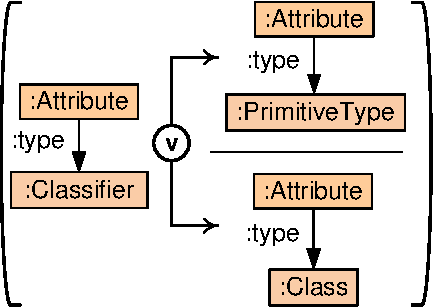
\includegraphics[width=.34\textwidth]{img/dc/constraints3.pdf}
}
The \code{type} edge is created by
rules \code{4:~TP2T} and \code{5:TC2T} in \cref{fig:rules}. The constraint on
the right is constructed by taking the atom with the \code{type} edge as the
premise and the disjunction of the embeddings of the atom into the right-hand-sides of both rules as the conclusion.
Analogously, the constraints for all other atoms $a \in Atoms(\TG_{S})$ over
source type graph $\TG_{S}$ in \cref{fig:mm} can be constructed.
\end{example}}


%%%%%%%%%%%%%%%%%%%%%%%%%%%%%%%%%%%%%%%%%%%%%%%%%%%%%%%%%%%%%%%%%%%%%%
%%%%%%%%%%%%%%%%%%%%%%%%%%%%%%%%%%%%%%%%%%%%%%%%%%%%%%%%%%%%%%%%%%%%%%
%%%%%%%%%%%%%%%%%%%%%%%%%%%%%%%%%%%%%%%%%%%%%%%%%%%%%%%%%%%%%%%%%%%%%%
%%%%%%%%%%%%%%%%%%%%%%%%%%%%%%%%%%%%%%%%%%%%%%%%%%%%%%%%%%%%%%%%%%%%%%
%%%%%%%%%%%%%%%%%%%%%%%%%%%%%%%%%%%%%%%%%%%%%%%%%%%%%%%%%%%%%%%%%%%%%%
%%%%%%%%%%%%%%%%%%%%%%%%%%%%%%%%%%%%%%%%%%%%%%%%%%%%%%%%%%%%%%%%%%%%%%
%%%%%%%%%%%%%%%%%%%%%%%%%%%%%%%%%%%%%%%%%%%%%%%%%%%%%%%%%%%%%%%%%%%%%%
%%%%%%%%%%%%%%%%%%%%%%%%%%%%%%%%%%%%%%%%%%%%%%%%%%%%%%%%%%%%%%%%%%%%%%
%%%%%%%%%%%%%%%%%%%%%%%%%%%%%%%%%%%%%%%%%%%%%%%%%%%%%%%%%%%%%%%%%%%%%%
%%%%%%%%%%%%%%%%%%%%%%%%%%%%%%%%%%%%%%%%%%%%%%%%%%%%%%%%%%%%%%%%%%%%%%
%%%%%%%%%%%%%%%%%%%%%%%%%%%%%%%%%%%%%%%%%%%%%%%%%%%%%%%%%%%%%%%%%%%%%%
%% app2.tex


% \newpage
% \section{Additional fragments to be possibly used in the paper}
% 
% ... now consider $\Lang_S \subseteq \Lang(TGG)\mid_{TG_S}$
% 
% This notion of domain-correctness can be achieved by showing $L(TGG)^T \subseteq L_T$.
% While this paper concentrates on the notion of domain-completeness, we define the task of providing a powerful method for showing the notion of domain-correctness as a challenge for future work and
% briefly describe how it can be handled with existing techniques.
% 
% 
% This paper presents a general method for validating and verifying this property in concrete application scenarios.
% We provide general results that ensure parts of the intermediate steps in general and 
% present in detail how the remaining parts can be solved including automated assistance by tool support.
% 
% This means that we have to show that $L_S \subseteq L(TGG)^S$.
% 
% \begin{math}
% \Lang_1=\Lang(TG_1,C_1) \Trans{Rest.} 
% \Lang_S=\restr{\Lang_1}{TG_S} \subseteq
% \Lang(TG_S,C_S) \subseteq \Lang(TG_S,TGG_S,C_{CT}) \subseteq \restr{\Lang(TGG)}{TG_S}
% \end{math}

% As in general,
% $L(TGG)^S \subseteq L(TR^S)$, we need to add constraints $C_2$ from $C_1'$ to
% $L(TR^S)$ leading to $L(TR^S+C_2)=\{G^S|\varnothing \xRightarrow{TR^{S*}} G^S, \forall c
% \in C_2.G^S \models c\}$ with $C_1' \implies C_2 \implies \varnothing$ until we
% hopefully get $L(TR^S+C_2) \subseteq L(TGG)^S$ without violating $L_S \subseteq
% L(TR^S+C_2)$ with the desired result $L_S \subseteq L(TGG)^S$ (cf. (1)).

% \subsection{Translation View of the Source Language}
% 
% Based on the concept of views in \cite{EEEP10}, a translation view of a language
% is defined as the restriction of the language to that subpart that is
% relevant for the model transformation.
% 
% \begin{definition}[Translation view]
% Given a language with constraints $L_{ATG,PC}$ and a triple type graph
% $ATG_S \leftarrow ATG_C \rightarrow ATG_T$ as a meta-model for the translation,
% then a translation view of that language is given by an injective morphism
% $v:ATG_S \rightarrow ATG$.
% \end{definition}
% 
% \begin{definition}[Restriction of models]
% Given a typed attributed graph $G$ with $G=(AG,t_{AG})$ typed over
% attributed type graph $ATG$ as a model and a translation view $v:ATG_S
% \rightarrow ATG$, then the restriction of the model $v^{<}(G)$
% with $v^{<}(G)=(AG_v,t_{AG_v})$
% is obtained by the pullback (1).
% \end{definition}
% 
% $
% 			\SelectTips{cm}{}
%     \xymatrix@R-4ex@C-4ex{ AG \ar[dd]_{t_{AG}} & & AG_v \ar[dd]^{t_{AG_v}}
%     \ar[ll] \\
%     			& (1) & \\
%                ATG & & ATG_S \ar[ll]^{v} }
% $
% 
% \begin{definition}[Restriction of constraints]
% Given a graph constraint $pc$ with $pc=((P, t_P) \xrightarrow{a} (C,
% t_C))$ typed over attributed type graph $ATG$ and a translation view $v:ATG_S
% \rightarrow ATG$, then the restriction of the constraint $v^{<}(pc)$ with
% $v^{<}(pc)=((P_v, t_{P_v}) \xrightarrow{a_v} (C_v,
% t_{C_v}))$ is obtained by pullbacks (1) and (2). Due to the universal
% property of pullback (2) with $v \circ t_{P_v}=t_P \circ p=t_C \circ a \circ p$,
% morphism $a_v$ exists such that $((P_v, t_{P_v}) \xrightarrow{a_v} (C_v,
% t_{C_v}))$ is a constraint over $ATG_S$.
% 
% The restriction of constraints is extended to the restriction $v^{<}(PC)$ of a
% set of constraints $PC$ with $v^{<}(PC)=\{v^{<}(pc) \mid pc \in PC\}$.
% \end{definition}
% 
% $
% 			\SelectTips{cm}{}
%     \xymatrix@R-4ex@C-4ex{
%     & P \ar[rr]^a \ar[dr]_{t_P} & & C \ar[dl]^{t_C} & \\
%     &  & ATG & & \\
%     & (1) & & (2) & \\
%     P_v \ar[uuur] \ar[rr]^{t_{P_v}} \ar@/_/[rrrr]_{a_v} & & ATG_S
%     \ar[uu]_{v} & & C_v \ar[uuul] \ar[ll]_{t_{C_v}} }
% $
% 
% \begin{definition}[Restriction of languages]
% Given a translation view $v:ATG_S \rightarrow ATG$ of language $L_{ATG,PC}$, the
% restriction of the language according to the view $v^{<}(L_{ATG,PC})$ is
% defined by the restriction of each graph and the restriction of each constraint
% of the language such that the restricted graphs fullfil the restricted
% constraints, i.e., $v^{<}(L_{ATG,PC})=\{v^{<}(G) \mid G \in L_{ATG,PC}, \forall c \in v^{<}(PC).G \models c\}$.
% \end{definition}
% 
% Note that in general, it is the fact that $v^{<}(G) \notin v^{<}(L_{ATG,PC})
% \text{ for some } G \in L_{ATG,PC}$.


%%%%%%%%%%%%%%%%%%%%%%%%%%%%%%%%%%%%%%%%%%%%%%%%%%%%%%%%%%%%%%%%%%%%%%
%%%%%%%%%%%%%%%%%%%%%%%%%%%%%%%%%%%%%%%%%%%%%%%%%%%%%%%%%%%%%%%%%%%%%%
%%%%%%%%%%%%%%%%%%%%%%%%%%%%%%%%%%%%%%%%%%%%%%%%%%%%%%%%%%%%%%%%%%%%%%
%%%%%%%%%%%%%%%%%%%%%%%%%%%%%%%%%%%%%%%%%%%%%%%%%%%%%%%%%%%%%%%%%%%%%%
%%%%%%%%%%%%%%%%%%%%%%%%%%%%%%%%%%%%%%%%%%%%%%%%%%%%%%%%%%%%%%%%%%%%%%
%%%%%%%%%%%%%%%%%%%%%%%%%%%%%%%%%%%%%%%%%%%%%%%%%%%%%%%%%%%%%%%%%%%%%%
%%%%%%%%%%%%%%%%%%%%%%%%%%%%%%%%%%%%%%%%%%%%%%%%%%%%%%%%%%%%%%%%%%%%%%
%%%%%%%%%%%%%%%%%%%%%%%%%%%%%%%%%%%%%%%%%%%%%%%%%%%%%%%%%%%%%%%%%%%%%%
%%%%%%%%%%%%%%%%%%%%%%%%%%%%%%%%%%%%%%%%%%%%%%%%%%%%%%%%%%%%%%%%%%%%%%
%%%%%%%%%%%%%%%%%%%%%%%%%%%%%%%%%%%%%%%%%%%%%%%%%%%%%%%%%%%%%%%%%%%%%%
%%%%%%%%%%%%%%%%%%%%%%%%%%%%%%%%%%%%%%%%%%%%%%%%%%%%%%%%%%%%%%%%%%%%%%
%% appendix.tex


For the rest of this section, we formalise the concepts of the proof idea of \cref{thm:C-extensionCompleteness} in order to finally prove \cref{thm:C-extensionCompleteness}.
We first show the equivalence of marking and transformation sequences with grammars for the case that the start graph is the empty graph in \cref{lem:equivalence-marking-emptySG} and that the start graph is an arbitrary graph in \cref{lem:equivalence-marking}.
Therefore, each graph that can be created via the rules of a given grammar $\GG$ can also be completely marked to $\True$ via the marking rules $m(\GG)$ of $\GG$ and vice versa.
%Given a graph $G$ with marking attributes, then by $(G^x \subseteq G)_{x \in \{\True, \False\}}$ we denote the subset of elements of $G$ (nodes, edges or attributes) that are annotated with a marking attribute of value $\True$ or $\False$, respectively.

\begin{lemma}[Equivalence of Marking and Transformation Sequence for empty Start Graph]
\label{lem:equivalence-marking-emptySG}
Let $\GG=(\varnothing,P)$ be a graph grammar with empty start graph $\varnothing$, a set $P$ of non-deleting rules and $m(\GG)$ be the set of derived marking rules of $\GG$. 
Let $G$ be a graph, then the following are equivalent for almost injective matches $m \in \morO$.
\begin{itemize}
	\item There exists a transformation $G \oplus \Att_G^\False \Trans{*} G \oplus \Att_{G_k}^\True \oplus \Att_{G \setminus G_k}^\False$ via marking rules $m(\GG)$.% with intermediate steps $(G'_i \Trans{(m_i,m(p_i))} G'_{i+1})$, where $m(p_i)=(L_i \xhookleftarrow{} K_i \xhookrightarrow{} R_i)$ and $\quotient{m_i}{L_i^{\False}}$ is type strict
	\item There exists a transformation $\varnothing \Trans{*} G_k$ via $P$ with injective embedding $f\colon G_k \to G$.% with intermediate steps $G_i \Trans{(m_i,p_i)} G_{i+1}$.
\envEndMarker
\end{itemize}
\end{lemma}

\begin{proof}
The proof is presented in \cref{sec-proofs:lem:equivalence-marking-emptySG}.
\end{proof}

% 
% 
% \noindent
% Using \cref{lem:equivalence-marking-emptySG} above, we now prove \cref{lem:equivalence-marking}.
% \\
% 
% \cref{lem:equivalence-marking} states the equivalence of marking rules
% $m(\GG)$ and the rules in $\GG$ in the sense that all graphs that can be
% completely marked to $\textbf{T}$ with rules $m(\GG)$ can also be created by
% the rules in $\GG$ and vice versa.

\begin{lemma}[Equivalence of Marking and Transformation Sequence]
\label{lem:equivalence-marking}
Let $\GG=(S,P)$ be a graph grammar with start graph $S$, a set $P$ of non-deleting rules and $m(\GG)$ be the set of derived marking rules of $\GG$. 
Let $G$ be a graph with inclusion $S \to G \in \M$, then the following are equivalent for almost injective matches $m \in \morO$.
\begin{itemize}
	\item There exists a transformation $G \oplus \Att_{S}^\True  \oplus \Att_{G\setminus S}^\False \Trans{*} G \oplus \Att_G^\True$ via marking rules $m(\GG)$.% with intermediate steps $G'_i \Trans{m_i,m(p_i)} G'_{i+1}$, where $m(p_i)=(L_i \xhookleftarrow{} K_i \xhookrightarrow{} R_i)$ and $\quotient{m_i}{L_i^{\False}}$ is type strict
	\item There exists a transformation $S \Trans{*} G$ via $P$.% with intermediate steps $G_i \Trans{p_i} G_{i+1}$.
\envEndMarker
\end{itemize}
\end{lemma}

\begin{proof}
The proof is presented in \cref{sec-proofs:lem:equivalence-marking}.
\end{proof}

\cref{def:bsplit} defines the binary split of a given graph $G$ into two sub-graphs which is extended to the general split of $G$ into its atoms $Atoms(G)$ in \cref{def:atomic-split} such that the gluing of the sub-graphs (atoms) yields $G$ again by \cref{lemma:union-subs,lemma:union-atoms}.
For proving \cref{lemma:union-atoms}, we show in \cref{lemma:split-nonatomic} that each non-atomic graph can be splitted.

%\vspace{1ex}
\parpic[r][r]{
$
\SelectTips{cm}{}
     \xymatrix@R-5ex@C-4ex{
     & \AG & \\
     \AG_1 \ar@{^{(}->}[ur]^{f'} & (1) & \AG_2 \ar@{_{(}->}[ul]_{g'} \\
     & \AG_0 \ar@{_{(}->}[ul]^{g} \ar@{^{(}->}[ur]_{f} &
     }
$
}
\vspace{-2ex}
\begin{definition}[Binary Split]
\label{def:bsplit}
\index{graph!binary split}
Let $\AG$ be a graph.
The set of \emph{binary splits} $BSplits(\AG)$ of $\AG$ into sub-graphs is given by co-spans of inclusions in \M:
\noindent
$
BSplits(\AG):= \{(\AG_1 \xhookrightarrow{f'} \AG \xhookleftarrow{g'} \AG_2) \mid $ 
(1) is  a pushout over inclusions $(f\colon \AG_0\xhookrightarrow{} \AG_2, g\colon \AG_0\xhookrightarrow{} \AG_1) \text{ with } f,f',g,g' \in \M, \AG \not\cong \AG_1, \AG\not\cong \AG_2\}$
%where $(\AG_1 \xhookrightarrow{f'_1} \AG \xhookleftarrow{g'_1} \AG_2) \sim (\AG'_1 \xhookrightarrow{f'_2} \AG \xhookleftarrow{g'_2} \AG'_2)$ if there exist isomorphisms $i_1\colon \AG_1 \to \AG'_1,i_2\colon \AG_2 \to \AG'_2$ and furthermore, $f'_1=f'_2 \circ i_1,g'_1=g'_2 \circ i_2$.
\envEndMarker
\end{definition}

\begin{corollary}[Gluing of Binary Split]
\label{lemma:union-subs}
Let $(\AG_1 \xhookrightarrow{f'} \AG \xhookleftarrow{g'} \AG_2) \in BSplits(\AG)$ be a binary split of $\AG$ into sub-graphs $\AG_1$ and $\AG_2$.
Then, there exist $\AG_0$ and a span of $\M$-morphisms $(\AG_1 \xhookleftarrow{g} \AG_0 \xhookrightarrow{f} \AG_2)$ such that (1) is a pushout.
\envEndMarker
\end{corollary}

% \begin{proof}
% Let $\AG=(G,D)$ and $(AG_i=(G_i,D))_{i \in \{0..2\}}$. By \cref{def:bsplit}, $(\AG,f',g')$ is a pushout over some inclusions $f\colon \AG_0
% \xhookrightarrow{} \AG_2$ and $g\colon \AG_0 \xhookrightarrow{} \AG_1$.
% Therefore, $f'(\AG_1) \cup g'(\AG_2) = \AG$. Furthermore, $f'_D=g'_D=id_D, f'_G(G_1)=G_1$ and $g'_G(G_2)=G_2$, i.e., $f'(\AG_1)=\AG_1$ and $g'(\AG_2)=\AG_2$. Therefore, $\AG_1 \cup \AG_2=\AG$.
% %\qed
% \end{proof}

\begin{lemma}[Binary Split of Non-Atomic Graphs]
\label{lemma:split-nonatomic}
Let $\AG$ be a graph that is not an atom, then $\AG$ can be splitted into sub-graphs $\AG_1$ and $\AG_2$ with $(\AG_1 \to \AG \gets \AG_2) \in BSplits(\AG)$.
\envEndMarker
\end{lemma}

\begin{proof}
We construct initial pushout (1) for $\id_\AG$ with $g' \in \M$.
Analogously, we construct initial pushout (2) for $g'$ with $f,f' \in \M$.
By \cref{sec-gt-M-adh,def:sec-gt-M-adh:hlr_props}, (2) is also a pullback, i.e., $g \in \M$ by $\M$-morphisms $g'$ are closed under pullbacks.
\begin{center}
$
\SelectTips{cm}{}
     \xymatrix@R-5ex@C-2ex{
     & & \AG & \\
     & \AG \ar[ur]^{\id_\AG} & (1) & \AG'' \ar[ul]_{} \\
     \AG_1 \ar[ur]^{f'} & (2) & \AG_2 \ar[ul]_{g'} \ar[ur]_{} & \\
     & \AG_0 \ar[ul]^{g} \ar[ur]_{f} & &
     }
$
\end{center}
Assumption $\AG$ is not an atom, \cref{def:atom} and $\M$-morphisms $f,g \in \M$ are closed under pushouts imply that there exists pushout (2) with $f,f',g,g' \in \M$ such that $\AG \not\cong \AG_1$ and $\AG \not\cong \AG_2$.
Thus according to \cref{def:bsplit}, there is $(\AG_1 \xhookrightarrow{f'} \AG \xhookleftarrow{g'} \AG_2) \in BSplits(\AG)$.
\end{proof}

Note that a graph $G$ may be splitted binary in different ways, possibly leading to several sets of atoms of $G$ in $Atoms(G)$.
However, for category $(\AGraphs_\ATGI,\M)$ all sets are isomorphic, i.e., only one set of atoms (decision path of binary splits) in $Atoms(G)$ need to be considered.

\begin{definition}[Atomic Split]
\label{def:atomic-split}
\index{graph!atomic split}
The \emph{set of atoms of a given graph $\AG$} is defined by $Atoms(\AG)$ as given below:
\newline
$
Atoms(\AG):= 
\begin{cases}
\{\{\AG\}\} & ,\AG \text{ is an atom} \\
\{A_1 \sqcup A_2 \mid (\AG_1 \xhookrightarrow{} \AG \xhookleftarrow{} \AG_2) \in BSplits(\AG), & ,\AG \text{ is not an atom} \\
A_1 \in Atoms(\AG_1),A_2 \in Atoms(\AG_2)\} & \hfill\envEndMarker
\end{cases}
$
\end{definition}

\parpic[r][r]{
$
\SelectTips{cm}{}
     \xymatrix@R-2ex@C-4ex{
     & PO_{k+1} & \\
     PO_k \ar@{^{(}->}[ur]^{f'_k} & (1) & a_{k+1} \ar@{_{(}->}[ul]_{g'_k} \\
     & G_k \ar@{_{(}->}[ul]^{g_k} \ar@{^{(}->}[ur]_{f_k} &
     }
$
}
\vspace{-2ex}
\begin{lemma}[Gluing of Atomic Split]
\label{lemma:union-atoms}
Let $G$ be a graph in $(\AGraphs_\ATGI,\M)$.
Then, there are atoms $(a_i)_{i \in \{1,\ldots,n\}} \in Atoms(G)$ and for all $(a_i)_{i \in \{1,\ldots,n\}} \in Atoms(G)$ there exist graphs $(G_j)_{1 \leq j \leq n-1}$ and pushouts $(PO_k +_{G_k} a_{k+1})_{k \in \{1,\ldots,n-1\}}$ with pushout objects $PO_{k+1}$ as depicted by pushout $(1)$ on the right with all morphisms in $\M$ and with $PO_1=a_1$ and induced morphisms $a_1 \trans{f'_1 \in \M} PO_2 \trans{f'_{n-1} \circ \ldots \circ f'_2 \in \M} PO_n \in \M$ and $a_{k+1} \trans{g'_k \in \M} PO_{k+1} \trans{f'_{n-1} \circ \ldots \circ f'_{k+1} \in \M} PO_n \in \M$ such that pushout object $PO_n$ is $G$.
\envEndMarker
\end{lemma}

\begin{proof}
Let $G$ be a graph.
\begin{description}
\item[Case ($G$ is an atom)] 
By construction \cref{def:atomic-split}, there is $\{G\} \in Atoms(G)=\{\{G\}\}$ with $n=1$, i.e., for all $(a_i)_{i \in \{1,\ldots,n\}} \in Atoms(G)$ the assumption holds with induced morphism $\id_G$.
\item[Case ($G$ is not an atom)]
By \cref{lemma:split-nonatomic}, there exists a binary split $(G_1 \trans{f'} G \transB{g'} G_2) \in BSplits(G)$.
By construction of binary splits in \cref{def:bsplit} with $G \not\cong G_1$, $G \not\cong G_2$ and injective $\M$-morphisms $f'$ and $g'$ it follows that $G_1$ and $G_2$ are smaller than $G$ on the graph part.
Therefore, analogously we can proceed with splitting $G_1$ and $G_2$ binary in $Atoms(G_1)$ and $Atoms(G_2)$ recursively and terminate in each decision path of binary splits when obtaining atoms.
Thus, there is $(a_i)_{i \in \{1,\ldots,n\}} \in Atoms(G)$.
Let $(a_i)_{i \in \{1,\ldots,n\}} \in Atoms(G)$ be the atoms of graph $G$.
By induction over the number $n$ of atoms:
\textbf{Basis.} For $n=2$, by construction there exists $(a_1 \trans{f'_1} G \transB{g'_1} a_2) \in BSplits(G)$ with $a_1,a_2$ being atoms, i.e., by \cref{lemma:union-subs} there exist $G_1$ and a span of $\M$-morphisms $(a_1 \transB{g_1} G_1 \trans{f_1} a_2)$ such that $(f'_1 \in \M,g'_1 \in \M)$ is a pushout over $(g_1,f_1)$ with induced morphisms $f'_1,g'_1 \in \M$ and with pushout object $PO_2=G$.
\textbf{Hypothesis.} There is $n$ such that the assumption holds.
\textbf{Step.} For $n+1$, note that in $(\AGraphs_\ATGI,\M)$, all decision paths of binary splits in $BSplits(G)$ lead to the same set of atoms $(a_i)_{i \in \{1,\ldots,n+1\}}$ up to isomorphism, i.e., we focus on that path where atoms are splitted from $G$ step-wise.
Let $G$ be binary splitted into $(G_1 \to G \gets a_{n+1}) \in BSplits(G)$ with atom $a_{n+1}$ and furthermore, let $(a_i)_{i \in \{1,\ldots,n\}} \in Atoms(G_1)$ and $(a_{n+1}) \in Atoms(a_{n+1})$.
By induction hypothesis, for $Atoms(G_1)$ there is pushout object $PO_n=G_1$ with induced morphisms in $\M$.
Analogously to the base case by \cref{lemma:union-subs}, for $(G_1 \trans{f'_n} G \transB{g'_n} a_{n+1}) \in BSplits(G)$ there is $G_n$ and pushout object $PO_{n+1}$ obtained by pushout $(f'_n \in \M,g'_n \in \M)=PO_n +_{G_n} a_{n+1}$ over $(g_n \in \M,f_n \in \M)$ with $PO_{n+1}=G$ and with induced morphisms in $\M$ by $\M$-composition with $f'_n \in \M$.
\end{description}
\end{proof}

Given a set of constraints $C$ that are designated for general satisfaction.
Then, \cref{lemma:closure-c-ext} states that for each atom $a$ of a graph $G$ which generally satisfies $C$, the extension of $a$ via $C$ is in $G$ again.
The result does not generally hold for constraints that are designated for initial satisfaction, since, atom $a$ may be extended at parts that are not covered by the satisfaction of the constraint potentially leading to extensions of $a$ that are not in G.

\begin{lemma}[Closure under $C$-Extensions of Atoms]
\label{lemma:closure-c-ext}
In $(\AGraphs_\ATGI,\M)$, let $C$ be a set of constraints that are designated for general satisfaction, $G \in \Lang(C)$ be a graph that generally satisfies $C$ and $a \in A \in Atoms(G)$ be an atom of $G$ with induced morphism $e\colon a \to G \in \M$ by \cref{lemma:union-atoms}.
Then, \emph{$G$ is closed under $C$-Extensions of $a$}, i.e., for all extensions $E \in Extensions(a,C)$ there is $a_E \in E$ with morphisms $e_1\colon a \to a_E \in \M, e_2\colon a_E \to G \in \M$ and $e=e_2 \circ e_1$.
\envEndMarker
\end{lemma}

\begin{proof}
The proof is presented in \cref{sec-proofs:lemma:closure-c-ext}.
\end{proof}

\cref{def:c-ext-set} extends the construction of $C$-extensions in \cref{def:C-extension} by defining the simultaneous extension of a set of graphs via a given set of constraints $C$.
This leads to the result in \cref{lem:union-ext-atoms} as an extension of \cref{lemma:union-atoms}.
Based on \cref{lemma:closure-c-ext}, \cref{lem:union-ext-atoms} states that given a graph $G$ which generally satisfies a given set of constraints $C$, then all simoultaneous extensions of the atoms of $G$ via $C$ contains a variant such that the gluing of the extended atoms yields graph $G$ again.

\begin{definition}[$C$-Extensions of Sets of Graphs]
\label{def:c-ext-set}
\index{$C$-extensions!sets of graphs}
Let $A$ be a set of graphs and $C$ be a set of constraints.
The set $SELECT_E(A,C)=\{f\colon A \to B \mid B=\bigcup_{a \in A}(Extensions(a,C)), \forall a \in A\colon f(a) \in Extensions(a,C)\}$ contains all functions $f$ that select for a given graph $a \in A$ an extension $E\in Extensions(a,C)$.
Let $f_E \in SELECT_E(A,C)$, then the set $SELECT_{a_E}(A,C,f_E)=\{f\colon A \to \bigcup_{E \in B}(E) \mid B=\bigcup_{a \in A}(Extensions(a,C)),\forall a \in A\colon f(a) \in f_E(a)\}$ contains all functions $f$ that select for a given graph $a \in A$ an extended graph $a_E \in f_E(a)$.
\envEndMarker 
\end{definition}

\begin{remark}
Note that for a graph $G$, the set of $C$-extensions $Extensions(G,C)$ may be infinite. Therefore, for a given set of graphs $A$, there may exists an infinite set of functions $SELECT_E(A,C)$.
Furthermore, a $C$-extension of a graph may be an infinite set of extended graphs. Therefore, for each selection $f_E \in SELECT_E(A,C)$, there may exists an infinite set of functions $SELECT_{a_E}(A,C,f_E)$.
\envEndMarker
\end{remark}

\begin{lemma}[Gluing of $C$-Extended Atoms]
\label{lem:union-ext-atoms}
In $(\AGraphs_\ATGI,\M)$, let $C$ be a set of constraints that are designated for general satisfaction, $G \in \Lang(C)$ be a graph that generally satisfies $C$ and $A=(a_i)_{i \in \{1,\ldots,n\}} \in Atoms(G)$ be the atoms of $G$.
Then, for all functions $f_E \in SELECT_E(A,C)$ that select a $C$-extension for each atom $a_i \in A$, there exists a function $f_{a_E} \in SELECT_{a_E}(A,C,f_E)$ that selects an extended atom for each atom $a_i \in A$ such that there exist graphs $(G^E_j)_{1 \leq j \leq n-1}$ and pushouts $(PO^E_k +_{G^E_k} f_{a_E}(a_{k+1}) = PO^E_{k+1})_{k \in \{1,\ldots,n-1\}}$ with pushout objects $PO^E_{k+1}$, all morphisms being in $\M$ and $PO^E_1=f_{a_E}(a_1)$ where (pushout object) $PO^E_n$ is $G$.
\envEndMarker 
\end{lemma}

\begin{proof}
The proof is presented in \cref{sec-proofs:lem:union-ext-atoms}.
\end{proof}

Note that in $(\AGraphs_\ATGI,\M)$, verifying domain completeness in \cref{thm:C-extensionCompleteness} via $C$-extension completeness in \cref{def:C-extensionCompleteness} is performed on the level of attributed graphs sharing the $\DSIG$-term algebra $T_\DSIG(X)$, since, effective atoms and their extensions share algebra $T_\DSIG(X)$ up to isomorphism by construction \cref{def:C-extension} with $e \in \M$ and \cref{sec-gt-M-adh,rem:sec-gt-M-adh:agraphs_atgi}.
In contrast to that, graphs of languages $\Lang(C)$ and $\Lang(\GG)$ may have concrete algebras with concrete values, in general (cf. general assumption of this section).
In order to close the algebra gap, in \cref{def:sec-dc-verification:instance_mor} we define instance morphisms $i\colon A \to B$ from attributed graphs $A$ with $\DSIG$-term algebra $T_\DSIG(X)$ to instance graphs $B$ with concrete algebras where concrete attribute values in $B$ are substituted by variables $x \in X$ in $A$ such that $i$ is an isomorphism on the graph part and injective for the data part of assigned attribute values.
Furthermore, we show that the verification of domain completeness on the term level does also hold for all (possibly infinitely many) instantiations to concrete values.
Therefore, given a set of productions $P$, in \cref{lem:atiti} we show that for each transformation $G \Trans{*} H$ via $P$ on the term level with instance morphism $i_H\colon H \to H'$ there is a corresponding transformation $G' \Trans{*} H'$ via $P$ with instance morphism $i_G\colon G \to G'$.
For proving \cref{lem:atiti}, based on the results in \cref{lem:comp_merge,lem:comp_e_mors} we first show in \cref{lem:ac_schema_sat_inst_mor} that a match satisfies an AC-schema if and only if the match extended by a given instance morphism satisfies the AC-schema.
\cref{lem:comp_merge} states that the successive merge over two morphisms is equivalent to the merge over the composition of both morphisms, i.e., in proofs for the satisfaction of AC-schemata, the merge over a composition of morphisms can be constructed step-wise (morphism by morphism successively).
For proving \cref{lem:comp_merge}, we additionally show the general results in \cref{lem:comp_o,lem:comp_epi,lem:m_adhesive_balanced,lem:pres_e_mor}.

\begin{definition}[Instance Morphism]
\label{def:sec-dc-verification:instance_mor}
\index{morphism!instance}
Let $DSIG=(S,OP)$ be a data signature.
In category $(\AGraphs_\ATGI,\M)$, \emph{a morphism $i\colon A \to B \in \E,\morO$ is an instance morphism}, if:
\begin{enumerate}
\item \label{item:sec-dc-verification:instance_mor:4}Attributed graph $A$ shares $\DSIG$-term algebra $T_\DSIG(X)$ with $X=(X_s)_{s \in S}$ being a family of infinite sets $X_s$ of variables for each sort $s \in S$,
\item \label{item:sec-dc-verification:instance_mor:5}attributed graph $B$ shares $\DSIG$-algebra $D_B$,
\item \label{item:sec-dc-verification:instance_mor:1}morphism $i$ is type strict,
\item \label{item:sec-dc-verification:instance_mor:2}all attribute values in $A$ are variables $x \in X$:$(\forall e \in E_j^A.t_j^A(e) \in X)_{j \in \{NA,EA\}}\}$, and
\item \label{item:sec-dc-verification:instance_mor:3}the data part of assigned attribute values is injective: $\forall d_1,d_2 \in D_A.(i_D(d_1)=i_D(d_2)) \wedge i_D(d_1) \in (t_{NA}^B(E_{NA}^B) \cup t_{EA}^B(E_{EA}^B)) \implies d_1=d_2$.
\envEndMarker
\end{enumerate}
\end{definition}

%#########################################################
\uncuttedversion{
Furthermore, we define the instances of an effective atom.
This is neccessary, since, effective atoms share the $\DSIG$-term algebra whereas graphs of a language (and its atoms) generally have algebras with concrete values which are considered as instances of terms (with variables).
In \cref{lemma:corr_atom_eatom}, we show that each effective atom $a \in EAtoms(C)$ is also an instance, i.e., $a \in \Inst(EAtoms(C))$.

\begin{definition}[Instance of Effective Atom]
\label{def:inst-effect-atom}
\index{atom!instance}
Given language $\Lang(C)$ over attributed type graph $\ATG$ and constraints $C$.
Let $a \in EAtoms(C)$ be an effective atom w.r.t. $\Lang(C)$ with morphism $f_a\colon a \to G \in \morO$ for some graph $G \in \Lang(C)$.% with $a=(G,D),\AG=(G',D')$.
The \emph{instance $\Inst_{f_a}(a)$ of atom $a$ w.r.t. $f_a$} is given by graph $O$ with extremal $\E$-$\M$ factorisation $m \circ e=f_a$ and $e\colon a \to O \in \E,m\colon O \to G \in \M$.
% $i_{f_a}(a)=a_I$ with
% $i_{f_a}(a):=(G'',D')$ and
% $G''=(f_a(V_G),f_a(E_G),V_D',f_a(E_{NA}),f_a(E_{EA}),(\quotient{s_i'}{f_a(E_i)},\quotient{t_i'}{f_a(E_i)})_{i
% \in \{G,NA,EA\}})$.
With $\Inst(a):=\{\Inst_{f_a}(a) \mid f_a\colon a \to G \in \morO,G \in \Lang(C)\}$ we denote the set of instances of atom $a$.
With $\Inst(EAtoms(C)):=\cup_{a \in EAtoms(C)}(\Inst(a))$ we denote the set of instances of effective atoms w.r.t. $\Lang(C)$.
\envEndMarker
\end{definition}

\begin{remark}
Note that for each (effective) atom $a$, an infinite set of morphisms $f_a\colon a \to G \in \morO$ with $G \in \Lang(C)$ may exist, i.e., each (effective) atom may have an infinite set of instances.
\envEndMarker
\end{remark}

\begin{lemma}[Correspondence of Atoms and Instances]
\label{lemma:corr_atom_eatom}
Given language $\Lang(C)$ over constraints $C$, and let $\AG \in EAtoms(C)$ be an effective atom w.r.t. $\Lang(C)$ with $i\colon \AG \to \AG' \in \M$ for some graph $\AG' \in \Lang(C)$.
Then, in category $(\AGraphs_\ATGI,\M)$ it holds that $\AG \in \Inst(EAtoms(C))$.
\envEndMarker
\end{lemma}

\begin{proof}
Let $f_a=i\colon \AG \to \AG' \in \M$ according to \cref{def:inst-effect-atom}, and $m \circ e=f_a$ be the extremal $\E$-$\M$ factorisation of $f_a$ with $e \in \E$ and $m \in \M$.
By $\M$-decomposition with $f_a,m \in \M$, it follows that $e \in \M$.
Therefore, according to \cref{sec-gt-M-adh,rem:sec-gt-M-adh:agraphs_atgi}, morphism $e$ is type strict, an isomorphism on the data part $e_D$ and injective on the graph part $e_G$.
Furthermore by $e \in \E$ and \cref{sec-gt-M-adh,rem:sec-gt-M-adh}, $e$ is an epimorphism, i.e., surjective, on the graph part $e_G$ implying further that $e$ is an isomorphism.
Thus, $\AG \in \Inst(EAtoms(C))$ up to isomorphism. 
\end{proof}


Analogously to \cref{def:inst-effect-atom}, we define the abstraction and instance of a graph.
This is neccessary, since, C-extension completeness verifies language inclusions on the level of attributed graphs sharing the term algebra with an infinite set of variables for each sort (abstract graphs).
In contrast to that, graphs of a language generally have algebras with concrete values, i.e., graphs of a language generally can be considered as instances of abstract graphs where variables are instantiated to concrete values.
Intuitively, the abstraction of an attributed graph $\AG^I=(G^I,D^I)$ with $DSIG$-algebra $D^I$ leads to an attributed graph $\AG=(G,T_{DSIG}(X))$ with a $DSIG$-term-algebra $T_{DSIG}(X)$ where concrete attribute values of $\AG^I$ are substituted by variables in $\AG$ such that all attributes with the same concrete value share the same variable and different concrete attribute values are substituted by different variables.
Therefore, each abstraction induces an instance morphism $i\colon \AG \to \AG^I$ that is an identity on the graph part and an isomorphism on the data part of assigned data values.
In order to obtain a unique instance morphism for each abstraction, the algebra $D^I$ must contain a designated abstraction element $*_s \in D_s^I$ for each sort $s$ to which unassigned variables are explicitly mapped. The unique evaluation of all other terms is given by the initiality of the term algebra $T_{DSIG}$.

\begin{definition}[Abstractable Graph]
\label{def:abstr-graph}
Let $DSIG=(S,OP)$ be a data signature. Let $\AG^I=(G^I,D^I)$ be an attributed graph with $DSIG$-algebra $D^I$. \emph{Graph $\AG^I$ is abstractable}, if $D^I$ contains a dedicated abstraction element $*_s \in D_s^I$ for each sort $s \in S$.
\envEndMarker
\end{definition}

In the following we define abstractions of graphs with concrete attribute values and instances of graphs.

\begin{definition}[Instance and Abstraction of Graphs]
\label{def:abstr-graphs}
Let $DSIG=(S,OP)$ be a data signature. Let $\AG^I=(G^I,D^I)$ be an abstractable attributed graph with $DSIG$-algebra $D^I$ and an abstraction element $*_s \in D_s^I$ for each $s \in S$.
\emph{The abstraction $\Abstr(\AG^I)$ of $\AG^I$} is defined by an instance morphism $\Abstr(\AG^I)=(i\colon \AG \to \AG^I)$
with $\AG=(G,D),D=T_{DSIG}(X),X=(X_s)_{s \in S}$ being a family of infinite sets $X_s$ of variables $(x^i_s)_{i \in \mathbb{N}}$ for each sort $s$ and $G=(V_{G}^I,V_{D},E_{G}^I,E_{NA}^I,E_{EA}^I,s_G^I,t_G^I,(s_j^I,t_j)_{j \in \{NA,EA\}})$ with $(\n{for all }e \in E_j^I \colon t_j(e) \in X)_{j \in \{NA,EA\}}\}$.
An instance morphism $i\colon \AG \to \AG^I$ is an attributed graph morphism without type refinements with $(i_{G,j})_{j \in \{V_G,E_G,E_{NA},E_{EA}\}}$ being identities, $\quotient{i_D}{t_{NA}(E_{NA}^I) \cup t_{EA}(E_{EA}^I)}$ and $\quotient{i_{G,V_D}}{t_{NA}(E_{NA}^I) \cup t_{EA}(E_{EA}^I)}$ being isomorphisms, and $(i_{D,s}(x_s^i)=*_s)_{s \in S}$ for all $x_s^i \in X \setminus (t_{NA}(E_{NA}^I) \cup t_{EA}(E_{EA}^I))$.
Let $A^I$ be a set of abstractable graphs. With $\Abstr(A^I)=\{\Abstr(\AG^I) \mid \AG^I \in A^I\}$ we denote the abstractions of graphs $A^I$.
Conversely, with $\Inst(\AG)=\{i\colon \AG \to \AG^I \mid i \n{ is an instance morphism} \}$ we denote the set of all instances of graph $\AG$.
\envEndMarker 
\end{definition}

\cref{def:compat-abstr} defines the situation in which the concrete values of the atomic sub-componenents of a graph are consistently abstracted to variables, i.e., identical (different) concrete values in different sub-components lead to identical (different) variables in their abstractions.

\begin{definition}[Compatible Abstraction of Atomic Sub-Components]
\label{def:compat-abstr}
Let $A^I=Atoms(\AG^I)$ be the atoms of an abstractable graph $\AG^I$.
\emph{The abstraction $\Abstr(A^I)$ of the atoms is compatible} with the abstraction $\Abstr(\AG^I)$ of $\AG^I$, if $\bigcup_{(i\colon A \to A^I) \in \Abstr(A^I)}(A)=\AG$ for $\Abstr(\AG^I)=(i\colon \AG \to \AG^I)$.
\envEndMarker 
\end{definition}
}
%####################################################################

\begin{lemma}[$\morO$-Morphisms are Closed Under De-Composition and Pushouts]
\label{lem:comp_o}
\label{lem:dec_o}
Let $f:\AG^1 \to \AG^2$, $g\colon \AG^2 \to \AG^3$ and $f'\colon \AG'^2 \to \AG^3$ be morphisms in $\AGraphs_{\ATGI}$.

\parpic[r][r]{
$
\SelectTips{cm}{}
     \xymatrix@R-5ex@C-5ex{
     AG^1 \ar@{->}[dd]^{} \ar@{->}[rr]^{f} & & AG^2 \ar@{->}[dd]^{g} \\
     & (1) & \\
     AG'^2 \ar@{->}[rr]^{f'} & & AG^3  
     }
$
}

\begin{enumerate}
  \item \label{item:lem:comp_o:1}If $f,g \in \morO$, then $g \circ f \in \morO$.
  \item Let $g \circ f = h$.
  \begin{enumerate}
    \item \label{item:lem:comp_o:2a}If $h \in \morO$, then $f \in \morO$.
    \item If $h \in \morO$ and graph part $f_S$ of $f$ is an isomorphism, then $g \in \morO$.
  \end{enumerate}
  \item For a given pushout (1), $f \in \morO$ implies $f' \in \morO$.\envEndMarkerB
\end{enumerate}
\end{lemma}

\begin{proof}
We proof the three facts as follows.
\begin{enumerate}
  \item The proof is given in \cite{DBLP:journals/tcs/GolasLEO12}, Thm. 7, item 7.
  \item
  \begin{enumerate}
    \item The proof is given in \cite{DBLP:journals/tcs/GolasLEO12}, Thm. 7, item 7.
    % With $g_S \circ f_S = h_S$,  $h_S$ being componentwise injective in $\cat{Sets}$ implies that $f_S$ is componentwise injective in $\cat{Sets}$, since, injective morphisms are closed under decomposition.
    % Therefore, $f \in \morO$.
    \item Let $f_S^{-1}\colon \AG^2 \to \AG^1$ be the inverse isomorphism of isomorphism $f_S$ with $f_S \circ f_S^{-1}=id_{\AG^2}$.
From $g_S \circ f_S = h_S$ we obtain $g_S \circ f_S \circ f_S^{-1} = h_S \circ f_S^{-1} \Leftrightarrow g_S \circ id_{\AG^2}=h_S \circ f_S^{-1} \Leftrightarrow g_S = h_S \circ f_S^{-1}$.
Since, $h_S, f_S^{-1}$ are componentwise injective in $\cat{Sets}$, it follows that $g_S$ is componentwise injective in $\cat{Sets}$, i.e., $g \in \morO$.
  \end{enumerate}
  \item Since (1) is a pushout, $f_S$ being componentwise injective in $\cat{Sets}$ implies that $f'_S$ is componentwise injective in $\cat{Sets}$ (cf. Fact 2.17, item 1 in \cite{Ehrig:2006:FAG:1121741}) and thus, $f' \in \morO$.
%  \qed
\end{enumerate}
\end{proof}

% \parpic[rf][r]{
% $
% \SelectTips{cm}{}
%      \xymatrix@R-3ex@C-3ex{
%      G_1 \ar@{->}[rr]^{h} \ar@{->}[dr]^{f} & & G_3 \\
%      & G_2 \ar@{->}[ur]^{g} &  
%      }
% $
% }
% \vspace{-2ex}
% \begin{lemma}[Decomposition of Isomorphisms]
% Let $f:G_1 \to G_2$, $g\colon G_2 \to G_3$ and $h\colon G_1 \to G_3$ be morphisms with $g \circ f = h$.
% \begin{enumerate*}
% \item If $h$ and $g$ are isomorphisms, then $f$ is an isomorphism.
% \item If $h$ and $f$ are isomorphisms, then $g$ is an isomorphism. 
% \end{enumerate*} 
% \envEndMarker
% \end{lemma}
% 
% \begin{proof}
% \begin{enumerate*}
% \item Let $g^{-1}\colon G_3 \to G_2$ be the inverse isomorphism of isomorphism $g$.
% Then, $g \circ f = h \Leftrightarrow g^{-1} \circ g \circ f = g^{-1} \circ h \Leftrightarrow id_{G_2} \circ f = g^{-1} \circ h \Leftrightarrow f = g^{-1} \circ h$.
% By the composition of isomorphisms $g^{-1}$ and $h$ it follows that $f$ is an isomorphism.
% \item Let $f^{-1}\colon G_2 \to G_1$ be the inverse isomorphism of isomorphism $f$.
% Then, $g \circ f = h \Leftrightarrow g \circ f \circ f^{-1}= h \circ f^{-1} \Leftrightarrow g \circ id_{G_1} = h \circ f^{-1} \Leftrightarrow g = h \circ f^{-1}$.
% By the composition of isomorphisms $h$ and $f^{-1}$ it follows that $g$ is an isomorphism.
% \end{enumerate*}
% \qed
% \end{proof}

% \begin{definition}[Merge$_{PO}$ over Morphism]
% Given a condition $\ac$ over $P$ and a morphism $b: P \rightarrow P'$, then based on \cref{def:merge morphism} $\Merge_{PO}(b,\ac)$ is a condition over $P'$ defined by
% \begin{itemize}
%   \item $\Merge_{PO}(b,\ac) = \exists(a',\Merge(b',\linebreak \ac'))$ if $\ac = \exists(a,\ac')$ and $(a',b',C')$ is a pushout over $(a,b,P)$,
%   \item $\Merge_{PO}(b,\ac) = \Merge(b,\ac)$, otherwise.
% \end{itemize}
% \envEndMarker
% \end{definition}
% 
% \begin{lemma}[Equivalence of $\Merge$ and $\Merge_{PO}$ Constructions]
% If b iso ($\morO$?) and $m \in \morO$, then $m \models \Merge(b,\ac) \Leftrightarrow m \models \Merge_{PO}(b,\ac)$.
% \envEndMarker
% \end{lemma}

%\vspace{-2ex}
\begin{lemma}[De-Composition of Pairs of Jointly Epimorphic Morphisms]\hfill
\label{lem:comp_epi}
\label{lem:decomp_epi}
\begin{center}
$
\SelectTips{cm}{}
     \xymatrix@R-5ex@C-3ex{
     G_0 \ar@{->}[dd]^{e} \ar@{->}[rr]^{e_2} & & G_1 \ar@{->}[dd]^{e_3} & & H \ar@{->}[ll]_{e_1} \\
     & (1) & & & \\
     G_2 \ar@{->}[rr]^{e_4} & & G & &  
     }
$
\end{center}
\begin{enumerate}
  \item Let $(e_1,e_2)$ and $(e_3,e_4)$ be pairs of jointly epimorphic morphisms and furthermore, (1) commutes.
        Then, $(e_3 \circ e_1,e_4)$ is a pair of jointly epimorphic morphisms.
  \item Let $(e_3 \circ e_1,e_4)$ be a pair of jointly epimorphic morphisms.
        Then, $(e_3,e_4)$ is a pair of jointly epimorphic morphisms.
  \item \label{lem:comp_epi:item:3} In the category $(\AGraphs_\ATGI,\M)$, let $(e_3,e_4)$ be a pair of jointly epimorphic morphisms, $e_4 \in \M$ and $e_1 \in \E$ be an extremal morphism w.r.t. $\M$.
        Then, $(e_3 \circ e_1,e_4)$ is a pair of jointly epimorphic morphisms.
  \item \label{lem:comp_epi:item:4} Let $(e_1,e_2)$ be jointly epimorphic and $e_3$ be an epimorphism.
        Then, $(e_3 \circ e_1,e_3 \circ e_2)$ is a pair of jointly epimorphic morphisms.
\envEndMarker 
\end{enumerate}
\end{lemma}

\begin{proof}
\begin{enumerate}
  \item We assume that (1) commutes and pairs $(e_1,e_2)$ and $(e_3,e_4)$ are jointly epimorphic.
        By the definition of jointly epimorphic morphisms, we have to show that for all graphs $G'$ and morphisms $f,g\colon G \to G'$ it holds that if $f \circ e_3 \circ e_1=g \circ e_3 \circ e_1$ $^{(*^1)}$ and $f \circ e_4=g \circ e_4$ $^{(*^2)}$, then $f=g$.
        Let $f,g\colon G \to G'$ be two morphisms with assumptions ($*^1$) and ($*^2$).
        Assumption ($*^2$) implies $f \circ e_4 \circ e=g \circ e_4 \circ e$.
        Since, (1) commutes it follows that $f \circ e_3 \circ e_2=g \circ e_3 \circ e_2$.
        By assumption ($*^1$) and $(e_1,e_2)$ being jointly epimorphic it follows that $f \circ e_3=g \circ e_3$.
        By assumption ($*^2$) and $(e_3,e_4)$ being jointly epimorphic it follows that $f=g$.
  \item We have to show for all morphisms $f,g$ that $f \circ e_3=g \circ e_3$ and $f \circ e_4=g \circ e_4$ implies $f=g$.
        Thus, $f \circ e_3=g \circ e_3 \implies f \circ e_3 \circ e_1=g \circ e_3 \circ e_1$.
        With $f \circ e_4=g \circ e_4$ it follows that $f=g$, since, $(e_3 \circ e_1,e_4)$ are jointly epimorphic.
  \item By assumption $e_4 \in \M$ and \cref{sec-gt-M-adh,rem:sec-gt-M-adh:agraphs_atgi}, $e_4$ is an isomorphism, i.e., an epimorphism, on the data part $e_{4,D}$.
        It remains to show that $(e_3 \circ e_1,e_4)$ are jointly epimorphic on the graph part.
        We assume the opposite.
        Then, there exists $g \in G$ with $g \not\in e_4(G_2)$ and $g \not\in e_3(e_1(H))$.
        The assumption that $(e_3,e_4)$ are jointly epimorphic implies that there exists $g' \in G_1$ with $e_3(g')=g$ but $g' \not\in e_1(H)$.
        Let $m \circ e'=e_1$ be the extremal $\E$-$\M$ factorisation of $e_1$  
        with $m\colon \ol{G_1} \to G_1 \in \M$.
        By the construction of the factorisation via the standard epi-mono factorisation on the graph structure part (cf. \cite{BEGG10}), it follows that $g' \not\in m(\ol{G_1})$ and therefore, $m$ is not an epi-(iso-)morphism.
        This contradicts with assumption $e_1 \in \E$ is extremal where $m \in \M$ implies that $m$ is an isomorphism (cf. \cref{def:EMFactorisation}).
  \item Given morphisms $g\colon G \to A$ and $h\colon G \to B$ with $g \circ e_3 \circ e_1=h \circ e_3 \circ e_1$ and $g \circ e_3 \circ e_2=h \circ e_3 \circ e_2$.
        By $(e_1,e_2)$ being jointly epimorphic, it follows that $g \circ e_3=h \circ e_3$ and $e_3$ being an epimorphism implies that $g=h$.
\end{enumerate}
\end{proof}

% \roundedYellowBox{
% \SelectTips{cm}{}
% $
% \xymatrix{
% P \ar[r]^a \ar[d]_b \ar@{}[dr]|{(1)}
% & C \ar[d]^{b'}
% \\
% P' \ar[r]_{a'}
% & C'
% }
% $
% }
% }

In general, it is not true that a monomorphism that is also an epimorphism is an isomorphism, since, the inverse morphism may not exist.
However, in $\M$-adhesive categories this assumption holds for a subclass $\M$ of monomorphisms as shown by \cref{lem:m_adhesive_balanced}.

\begin{lemma}[Relationship between $\M$-, Epi- and Iso-Morphisms in $\M$-adhesive Categories]
\label{lem:m_adhesive_balanced}
Given an $\M$-adhesive category $(\cat{C},\M)$, then any $\M$-morphism that is also an epimorphism is an isomorphism. 
\envEndMarker
\end{lemma}
\begin{proof}
The proof is based on the proof of Lemma 4.9 in \cite{Lack99adhesiveand} for adhesive categories.
Let (1) be a commuting diagram with epimorphism $m\colon A \to B \in \M$.
From $m$ being an epimorphism, it follows that (1) is a pushout, since, diagram (1) already commutes.
It remains to show the universal pushout property. 
For all morphisms $b_1,b_2\colon B \to \underline{B}$ with $b_1 \circ m=b_2 \circ m$ it follows that $b_1=b_2$ by the definition of epimorphisms.
Furthermore, there exists a morphism $\underline{b}=b_1=b_2$ with $\underline{b} \circ id_B=b_1 \circ id_B=b_2 \circ id_B=b_1=b_2$.
Moreover, $\underline{b}$ is unique.
Assume that there exists a morphism $\underline{b'}\colon B \to \underline{B}$ with $\underline{b'} \neq \underline{b}$ and $\underline{b'} \circ id_B=\underline{b'}=b_1=b_2=\underline{b}$ leading to a contradiction.

Since, (1) is a pushout along $\M$-morphism $m$, (1) is also a pullback (cf. Theorem 4.26, item 1 in \cite{Ehrig:2006:FAG:1121741}).
By the universal pullback property, there exists the inverse morphism $m^{-1}\colon B \to A$ with $m \circ m^{-1}=id_B$.
Furthermore, $m \circ id_A=id_B \circ m=m \circ m^{-1} \circ m$ and $m \in \M$ being a monomorphism by the definition of class $\M$ (cf. Def. 4.13 in \cite{Ehrig:2006:FAG:1121741}) implies $m^{-1} \circ m=id_A$.
\begin{center}
\begin{tikzpicture}[]
\fill (-3,1) node[inner sep=1pt] (Au) {$B$};
\fill (-2,0) node[inner sep=1pt] (A) {$A$};
\fill (0,0) node[inner sep=1pt] (B) {$B$};
\fill (0,-1) node[inner sep=1pt] (B'') {$B$};
\fill (-2,-1) node[inner sep=1pt] (B') {$B$};
\fill (1,-2) node[inner sep=1pt] (Bu) {$\underline{B}$};
\fill (-1,-.5) node[inner sep=1pt] (D1) {$(1)$};
%
{
\pgfsetarrowsend{latex}
\draw (B) -> node[right,inner sep=1pt]{$\scriptstyle{id_B}$} (B'');
\draw (B') -> node[below,inner sep=1pt]{$\scriptstyle{id_B}$} (B'');
\draw (Au) -> node[right,inner sep=5pt]{$\scriptstyle{m^{-1}}$} (A);
\draw (Au) edge[bend right=25] node[left,inner sep=1pt]{$\scriptstyle{id_B}$} (B');
\draw (Au) edge[bend left=25] node[right,inner sep=5pt]{$\scriptstyle{id_B}$} (B);
\draw (B'') -> node[above,inner sep=1pt]{$\scriptstyle{\underline{b}}$} (Bu);
\draw (B') edge[bend right=25] node[left,inner sep=5pt]{$\scriptstyle{b_1}$} (Bu);
\draw (B) edge[bend left=25] node[right,inner sep=1pt]{$\scriptstyle{b_2}$} (Bu);

\pgfsetarrows{right hook->>}
\draw (A) -> node[above,inner sep=1pt]{$\scriptstyle{m}$} (B);
\draw (A) -> node[left,inner sep=1pt]{$\scriptstyle{m}$} (B');
}
\end{tikzpicture}
\end{center}
%\qed
\end{proof}

\begin{lemma}[Preservation of Extremal Morphisms]\xqed{}
\label{lem:pres_e_mor}
\begin{minipage}{.68\textwidth}
Let $(\cat{C},\M)$ be an $\M$-adhesive category and $e \in \E$ be an extremal morphism with respect to $\M$ in $\cat{C}$.
Given diagram (1), if (1) commutes and morphisms $(a',e')$ are jointly epimorphic, then morphism $e'$ is an extremal morphism with respect to $\M$ in $\cat{C}$, i.e., $e' \in \E$.
\envEndMarker
\end{minipage}
\hfill
\begin{minipage}{0.3\textwidth}
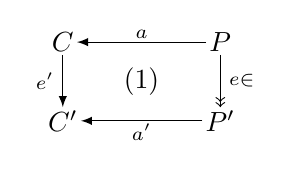
\begin{tikzpicture}[]
\fill (0,0) node[inner sep=1pt] (P) {$P$};
\fill (0,-1) node[inner sep=1pt] (P') {$P'$};
\fill (-2,0) node[inner sep=1pt] (C) {$C$};
\fill (-2,-1) node[inner sep=1pt] (C') {$C'$};
\fill (-1,-.5) node[inner sep=1pt] (D1) {$(1)$};
%
{
\pgfsetarrowsend{latex}
\draw (P) -> node[above,inner sep=1pt]{$\scriptstyle{a}$} (C);
\draw (P') -> node[below,inner sep=1pt]{$\scriptstyle{a'}$} (C');
\draw (C) -> node[left,inner sep=3pt]{$\scriptstyle{e'}$} (C');

\pgfsetarrows{->>}
\draw (P) -> node[right,inner sep=3pt]{$\scriptstyle{e \in \E}$} (P');
}
\end{tikzpicture}
\end{minipage}
\end{lemma}

\begin{proof}
Let $(\cat{C},\M)$ be an $\M$-adhesive category, $e \in \E$, $e' \circ a=a' \circ e$ and $(a',e')$ be jointly epimorphic.
By the definition of extremal morphisms (cf. \cref{def:EMFactorisation}), morphism $e'$ is extremal ($e' \in \E$) if for all morphisms $c,c'$ with $c' \circ c=e'$ it is true that $c' \in \M$ implies $c'$ is an isomorphism.
Given a decomposition of $e'\colon C \to C'$ with morphisms $c\colon C \to \underline{C}$, $c'\colon \underline{C} \to C'$, $c' \circ c=e'$ and $c' \in \M$.
Since pullbacks exist along $M$-morphisms in $\cat{C}$ and $\M$-morphisms are closed under pullbacks (cf. Def. 4.9 in \cite{Ehrig:2006:FAG:1121741}), we can construct pullback $(PB)$ along $c' \in \M$ with $p' \in \M$.
By the universal pullback property and assumption $e' \circ a=c' \circ c \circ a=a' \circ e$, there exists morphism $p\colon P \to \underline{P}$ with $\underline{a} \circ p=c \circ a$ and $p' \circ p=e$.
Thus, $e \in \E$, $p' \circ p=e$ and $p' \in \M$ implies $p'$ is an isomorphism (cf. \cref{sec-gt-M-adh,def:EMFactorisation}).
It remains to show that $c'$ is an epimorphism.
By $c' \in \M$ and \cref{lem:m_adhesive_balanced} it would follow that $c'$ is an isomorphisms and thus, $e'$ is extremal.
Morphism $c'$ is an epimorphism means that for all morphisms $f,g\colon C' \to G$ it holds that $f \circ c'=g \circ c'$ implies $f=g$ (cf. Def. 2.13  in \cite{Ehrig:2006:FAG:1121741}).
Let $f \circ c'=g \circ c'$.
Therefore, $f \circ e'=f \circ c' \circ c=g \circ c' \circ c=g \circ e'$ $^{(*^1)}$.
Furthermore, $f \circ a'=f \circ a' \circ id_{P'}=f \circ a' \circ p' \circ p'^{-1}= f \circ c' \circ \underline{a} \circ p'^{-1}=g \circ c' \circ \underline{a} \circ p'^{-1}=g \circ a' \circ p' \circ p'^{-1}=g \circ a'$ $^{(*^2)}$ with $p'^{-1}$ being the inverse morphism of isomorphism $p'$.
Since, $(a',e')$ are jointly epimorphic, $(*^1)$ and $(*^2)$ implies $f=g$.
Therefore, $c'$ is an epimorphism and by \cref{lem:m_adhesive_balanced} $c'$ is an isomorphism and thus, $e' \in \E$.

\begin{center}
\begin{tikzpicture}[]
\fill (0,0) node[inner sep=1pt] (P) {$P$};
\fill (0,-3) node[inner sep=1pt] (P') {$P'$};
\fill (-4,0) node[inner sep=1pt] (C) {$C$};
\fill (-4,-3) node[inner sep=1pt] (C') {$C'$};
\fill (-3,-1.5) node[inner sep=1pt] (Cu) {$\underline{C}$};
\fill (-1,-1.5) node[inner sep=1pt] (Pu) {$\underline{P}$};
\fill (-2,-2.2) node[inner sep=1pt] (PB) {$(PB)$};
\fill (-6,-3) node[inner sep=1pt] (G) {$G$};
%
{
\pgfsetarrows{-latex}
\draw (P) -> node[above,inner sep=1pt]{$\scriptstyle{a}$} (C);
\draw (P') -> node[above,inner sep=1pt]{$\scriptstyle{a'}$} (C');
\draw (C) -> node[right,inner sep=1pt]{$\scriptstyle{c}$} (Cu);
\draw (P) -> node[left,inner sep=1pt]{$\scriptstyle{p}$} (Pu);
\draw (Pu) -> node[above,inner sep=1pt]{$\scriptstyle{\underline{a}}$} (Cu);
\draw (C) -> node[left,inner sep=3pt]{$\scriptstyle{e'}$} (C');
\draw (C'.north west) -> node[above,inner sep=1pt]{$\scriptstyle{f}$} (G.north east);
\draw (C'.south west) -> node[below,inner sep=1pt]{$\scriptstyle{g}$} (G.south east);

\pgfsetarrows{->>}
\draw (P) -> node[right,inner sep=3pt]{$\scriptstyle{e \in \E}$} (P');

\pgfsetarrows{right hook-latex}
\draw (Cu) -> node[right,inner sep=1pt]{$\scriptstyle{c'}$} (C');
\draw (Pu) -> node[left,inner sep=1pt]{$\scriptstyle{p'}$} (P');
}
\end{tikzpicture}
\end{center}
%\qed
\end{proof}

In general, the merge of a condition over two morphisms successively is not equivalent to the merge of the condition over the composition of both morphisms as illustrated by \cref{ex:merge_comp}.
\cref{lem:comp_merge} defines sufficient conditions under which the equivalence holds. 

\begin{example}[General Equivalence of Successive Merge and Merge over Composition]
\label{ex:merge_comp}
\cref{fig:merge_comp} illustrates the merge $\Merge(b_2 \circ b_1,\ac_P)$ of condition $\ac_P=\exists(a\colon P \to C,\true)$ over the composition of morphisms $b_1$ and $b_2$ as well as the merge $\Merge(b_2,\Merge(b_1,\ac_P))$ of $\ac_P$ over morphisms $b_1$ and $b_2$ successively.
The example serves as a counterexample for showing that the merge over a composition of two morphisms is not equivalent to the merge over both morphisms successively, in general.
For simplicity, the graphs in the example share no algebras and all nodes are of type $T0$.
The nodes are mapped to nodes of the same name along morphisms.
The merge over composition is constructed by the commuting outer diagram with morphisms $b' \in \morO$ and $a'' \in \M$ and results in condition $\exists(a''\colon P'' \to C'',\true)=\Merge(b_2 \circ b_1,\ac_P)$.
The successive merge results in condition $\false=\Merge(b_2,\Merge(b_1,\ac_P))$.
Diagram $(1)$ can be constructed for the first merge $\Merge(b_1,\ac_P)$ of $\ac_P$ over morphism $b_1$ but diagram $(2)$ does not exist for the subsequent merge over $b_2$, since, the merge construction requires that the morphism between graphs $C'$ and $C''$ must be an $\morO$-morphism where the nodes are mapped injectively (cf. \cref{def:merge morphism}) but no $\morO$-morphism can be found.
This results in condition $\false$ for the sucessive merge (cf. \cref{rem:mom}).
Thus, $\Merge(b_2,\Merge(b_1,\ac_P)) \not\equiv \Merge(b_2 \circ b_1,\ac_P)$, i.e., the merge of a condition over two morphisms successively is not equivalent to the merge of the condition over the composition of both morphisms, in general.
The same situation arises if $\ac_P$ is not in $\M$-normal form ($a \not\in \M$) and therefore, $a$ identifies elements that are not identified by $b_1$ but by $b_2$ and therefore, $(1)$ cannot be constructed resulting into $\Merge(b_1,\ac_P)=\false \Rightarrow \Merge(b_2,\Merge(b_1,\ac_P))=\false \not\equiv \Merge(b_2 \circ b_1,\ac_P)$ (cf. \cref{rem:mom}).
\envEndMarker

\begin{figure}[htb]
\begin{center}
\scalebox{1.0}{\begin{tikzpicture}[]

\node (P) [box]{ 
			\begin{tikzpicture}
			\node(title) {$P$}; 
			\node (P1) [below of=title, yshift=.5cm, anchor=west, normal, rectangle split parts=1] {1:T0};
			\end{tikzpicture}
};
\node (C) [right=of P, box, xshift=2cm]{ 
			\begin{tikzpicture}
			\node(title) {$C$}; 
			\node (C1) [below of=title, yshift=.5cm, anchor=west, normal, rectangle split parts=1] {1:T0};
			\end{tikzpicture}
};
\node (P') [below=of P, yshift=.5cm, box]{ 
			\begin{tikzpicture}
			\node(title) {$P'$}; 
			\node (P'1) [below of=title, yshift=.5cm, anchor=west, normal, rectangle split parts=1] {1:T0};
			\node (P'2) [right of=P'1, anchor=west, normal, rectangle split parts=1] {2:T0};       
			\end{tikzpicture}
};
\node (C') [below=of C, yshift=.5cm, box]{ 
			\begin{tikzpicture}
			\node(title) {$C'$}; 
			\node (C'1) [below of=title, yshift=.5cm, anchor=west, normal, rectangle split parts=1] {1:T0};
			\node (C'2) [right of=C'1, anchor=west, normal, rectangle split parts=1] {2:T0};
			\end{tikzpicture}
};
\node (P'') [below=of P', yshift=.5cm, box]{ 
			\begin{tikzpicture}
			\node(title) {$P''$}; 
			\node (P'1) [below of=title, yshift=.5cm, anchor=west, normal, rectangle split parts=1] {1,2:T0};
			\end{tikzpicture}
};
\node (C'') [below=of C', yshift=.5cm, box]{ 
			\begin{tikzpicture}
			\node(title) {$C''$}; 
			\node (C'1) [below of=title, yshift=.5cm, anchor=west, normal, rectangle split parts=1] {1,2:T0};
			\end{tikzpicture}
};

\fill (2.2,-.85) node[inner sep=1pt] (rect1) {$(1)$};
\fill (2.2,-2.8) node[inner sep=1pt] (rect2) {$(2)$};

{
\pgfsetarrowsend{latex}
\draw[thick] (P) ->node[left,inner sep=5pt]{$b_1$} (P');
\draw[thick] (P') ->node[left,inner sep=5pt]{$b_2$} (P'');

\pgfsetarrows{*-latex}
\draw[thick] (C) ->node[right,inner sep=5pt]{$b'_1 \in \morO$} (C');
\draw (C) edge[bend left=85] node[right,inner sep=5pt]{$b' \in \morO$} (C'');
\draw[thick] (C') edge[] node[right, inner sep=5pt]{$\nexists \in \morO$} (C'');

\pgfsetarrows{right hook-latex}
\draw[thick] (P) ->node[above,inner sep=1pt]{$a \in \M$} (C);
\draw[thick] (P') ->node[above,inner sep=1pt]{$a' \in \M$} (C');
\draw[thick] (P'') ->node[above,inner sep=1pt]{$a'' \in \M$} (C'');
}       

\end{tikzpicture}}
\caption{\label{fig:merge_comp}Counterexample for General Equivalence}
\end{center}
\end{figure}

\end{example}

\begin{lemma}[Equivalence of Successive Merge and Merge over Composition]
\label{lem:comp_merge}
In $(\AGraphs_\ATGI,\M)$, let $\ac_P$ be a condition over $P$ in $\M$-normal form.
Furthermore, let $b_1\colon P \to P'$ and $b_2\colon P' \to P''$ be morphisms from $P$ or
$P'$ to some $P'$ or $P''$, respectively.
Furthermore, let $b_1 \in \E$. 
It holds that $\Merge(b_2,Merge(b_1,\ac_P)) \equiv \Merge(b_2 \circ b_1,\ac_P)$.
\envEndMarker
\end{lemma}
\begin{center}
\begin{tikzpicture}[]
\fill (.5,1.7) node[inner sep=1pt] (P) {$P$};
\fill (0.5,.75) node[inner sep=1pt] (P') {$P'$};
\fill (0.5,-.2) node[inner sep=1pt] (P'') {$P''$};
\fill (-.1,1.7) node [isosceles triangle, fill=gray!25,draw,minimum width=0.4cm, inner sep=1pt] (t) {};
\fill (-.1,.75) node [isosceles triangle, fill=gray!25,draw,minimum width=0.4cm, inner sep=1pt] (t) {};
\fill (-.1,-.2) node [isosceles triangle, fill=gray!25,draw,minimum width=0.4cm, inner sep=1pt] (t) {};
\fill (-.6,1.7) node[inner sep=1pt] {$\ac_P$};
\fill (-1.45,.75) node[inner sep=1pt] {$\Merge(b_1,\ac_P)$};
\fill (-4,-.2) node[inner sep=1pt] {$\Merge(b_2 \circ b_1,\ac_P) \equiv \Merge(b_2, \Merge(b_1,\ac_P))$};
%
{
\pgfsetarrowsend{latex}
\draw (P') -> node[left,inner sep=1pt]{$\scriptstyle{b_2}$} (P'');

\pgfsetarrows{->>}
\draw (P) -> node[left,inner sep=1pt]{$\scriptstyle{b_1 \in \E}$} (P');
}
\end{tikzpicture}
\end{center}
\begin{proof}
The proof is presented in \cref{sec-proofs:lem:comp_merge}.
\end{proof}

\begin{lemma}[Composition of Extremal Morphisms]
\label{lem:comp_e_mors}
Let $(\cat{C},\M)$ be an $\M$-adhesive category and $e_1\colon A \to B,e_2\colon B \to C \in \E$ be extremal morphisms with respect to $\M$ in $\cat{C}$.
The composition $e_2 \circ e_1$ is also an extremal morphism with respect to $\M$ in $\cat{C}$ ($e_2 \circ e_1 \in \E$).
\envEndMarker
\end{lemma}
\begin{proof}
Let $e_1,e_2 \in \E$ and $m \circ f$ be a factorisation of $e_2 \circ e_1$ with $m \circ f=e_2 \circ e_1$ and $m \in \M$.
It remains to show that $m$ is an isomorphism (cf. \cref{def:EMFactorisation}).
We can construct pullback (1) along $m \in \M$ with $m_1 \in \M$, since, pullbacks exist along $\M$-morphisms in $\cat{C}$ and $\M$-morphisms are closed under pullbacks by definition (cf. Def. 4.13, item 2 in \cite{Ehrig:2006:FAG:1121741}).
By the universal pullback property we obtain morphism $f_1$ with $m_1 \circ f_1=e_1$.
Thus, the assumption $e_1 \in \E$ with $m_1 \in \M$ imply that $m_1$ is an isomorphism (cf. \cref{def:EMFactorisation}).
(1) being a pullback implies $e_2 \circ m_1=m \circ f_2 \stackrel{m_1\ iso}{\implies} e_2 \circ m_1 \circ m_1^{-1}=m \circ f_2 \circ m_1^{-1} \Leftrightarrow e_2 \circ id_B=m \circ f_2 \circ m_1^{-1} \Leftrightarrow e_2=m \circ f_2 \circ m_1^{-1}$.
Thus, the assumptions $e_2 \in \E$ and $m \in \M$ imply that $m$ is an isomorphism (cf. \cref{def:EMFactorisation}).
\begin{center}
\begin{tikzpicture}[]
\fill (0,0) node[inner sep=1pt] (A) {$A$};
\fill (3,0) node[inner sep=1pt] (B) {$B$};
\fill (6,0) node[inner sep=1pt] (C) {$C$};
\fill (3,2) node[inner sep=1pt] (B') {$\ol{B}$};
\fill (3,1) node[inner sep=1pt] (D) {$D$};
\fill (4,.7) node[inner sep=1pt] (1) {$(1)$};
\fill (2.35,.4) node[inner sep=1pt] (eq) {$(=)$};
%
{
\pgfsetarrows{-latex}
\draw (A) -> node[above,inner sep=1pt]{$\scriptstyle{f}$} (B');
\draw (D) -> node[right,inner sep=1pt]{$\scriptstyle{f_2}$} (B');
\draw (A) -> node[above,inner sep=1pt]{$\scriptstyle{f_1}$} (D);
\pgfsetarrows{->>}
\draw (A) -> node[above,inner sep=1pt]{$\scriptstyle{e_1 \in \E}$} (B);
\draw (B) -> node[above,inner sep=1pt]{$\scriptstyle{e_2 \in \E}$} (C);
\pgfsetarrows{right hook-latex}
\draw (B') -> node[right,inner sep=5pt]{$\scriptstyle{m \in \M}$} (C);
\draw (D) -> node[right,inner sep=1pt]{$\scriptstyle{m_1}$} (B);
}
\end{tikzpicture}
\end{center}
%\qed
\end{proof}

\cref{lem:ac_schema_sat_inst_mor} states that for a given match $m\colon P \to G$ and instance morphism $i\colon G \to G'$, $m$ satisfies the AC-schema $\ol{\ac}_P$ of a given condition $\ac_P$ in $\M$-normal form ($m \models \ol{\ac}_P$) if and only if $m$ extended by $i$ satisfies $\ol{\ac}_P$ ($i \circ m \models \ol{\ac}_P$).
For direction $i \circ m \models \ol{\ac}_P \Rightarrow m \models \ol{\ac}_P$, the restriction to conditions in $\M$-normal form becomes essential as illustrated by \cref{ex:schema_sat} leading to the restriction to application conditions in $\M$-normal form in \cref{lem:atiti}.

\begin{example}[AC-schema Satisfaction by Instance Morphisms for General Conditions]
\label{ex:schema_sat}
For category $(\AGraphs_\ATGI,\M)$, \cref{fig:schema_sat} illustrates that given a condition $\ac_P=\exists(a\colon P \to C,\true)$ that is not in $\M$-normal form, then it may be true that $i \circ m\models \ol{\ac}_P$ but $\neg(m \models \ol{\ac}_P)$.
\begin{figure}[htb]
\begin{center}
\scalebox{1.0}{\begin{tikzpicture}[]

\node (P) [box]{ 
			\begin{tikzpicture}
			\node(title) {$P$}; 
			\node (Item) [below=of title, anchor=west, yshift=1cm]
					{
							$\varnothing$
					};
			\end{tikzpicture}
};
\node (C) [right=of P, box, xshift=7.5cm]{ 
			\begin{tikzpicture}
			\node(title) {$C$}; 
			\node (Item) [below=of title, anchor=west, normal, yshift=.35cm]
					{
							1:T0
							\nodepart{second}
							$\begin{array}{l}
							value=x\\						
							\end{array}$
					};
			\end{tikzpicture}
};
\node (G) [below=of P, yshift=-1cm, box]{ 
			\begin{tikzpicture}
			\node(title) {$G$}; 
			\node (Item) [below=of title, anchor=west, normal, yshift=.35cm]
					{
							1:T0
							\nodepart{second}
							$\begin{array}{l}
							value=x					
							\end{array}$
					};
			\end{tikzpicture}
};
\node (P2) [right=of G, xshift=1cm, yshift=0cm, box]{ 
			\begin{tikzpicture}
			\node(title) {$P_2$}; 
			\node (Item) [below=of title, anchor=west, yshift=1cm]
					{
							$\varnothing$
					};
			\end{tikzpicture}
};
\node (C2) [right=of P2, xshift=1.7cm, box]{ 
			\begin{tikzpicture}
			\node(title) {$C_2$}; 
			\node (Item) [below=of title, anchor=west, normal, yshift=.35cm]
					{
							1:T0
							\nodepart{second}
							$\begin{array}{l}
							value=a					
							\end{array}$
					};
			\end{tikzpicture}
};
\node (G^I) [below=of G, box, yshift=-1cm]{ 
			\begin{tikzpicture}
			\node(title) {$G^I$}; 
						\node (Item) [below=of title, anchor=west, normal, yshift=.35cm]
					{
							1:T1
							\nodepart{second}
							$\begin{array}{l}
							value=1						
							\end{array}$
					};
			\end{tikzpicture}
};
\node (P3) [right=of G^I, xshift=1cm, yshift=0cm, box]{ 
			\begin{tikzpicture}
			\node(title) {$P_3$}; 
			\node (Item) [below=of title, anchor=west, yshift=1cm]
					{
							$\varnothing$
					};
			\end{tikzpicture}
};
\node (C3) [right=of P3, xshift=1.7cm, box]{ 
			\begin{tikzpicture}
			\node(title) {$C_3$}; 
			\node (Item) [below=of title, anchor=west, normal, yshift=.35cm]
					{
							1:T1
							\nodepart{second}
							$\begin{array}{l}
							value=1						
							\end{array}$
					};
			\end{tikzpicture}
};
\node (D1) [right=of P, xshift=3.5cm, yshift=-1.5cm]{(1)};
\node (D2) [right=of G^I, xshift=1.5cm, yshift=-.9cm]{(2)};
{
\pgfsetarrowsend{latex}
\draw[thick] (C3.south west) edge[bend left=15] node[fill=white,inner sep=5pt]{$\exists q' \in \M$} (G^I.south east);
\draw[thick] (C2.south west) edge[bend left=15] node[fill=white,inner sep=5pt,xshift=1cm]{$\nexists q \in \M$} (G.south east);
\draw[thick] (P) ->node[fill=white,inner sep=1pt]{$a\colon \begin{array}{l}
							x \mapsto x\\
							y \mapsto z\\
							z \mapsto z						
							\end{array}$} (C);

\pgfsetarrows{*-latex}
\draw[thick] (P) ->node[left,inner sep=1pt]{$m \in \morO\colon \begin{array}{l}
							x \mapsto a\\
							y \mapsto y\\
							z \mapsto z						
							\end{array}$} (G);
\draw[thick] (G) ->node[left,inner sep=1pt]{$i \in \morO\colon \begin{array}{l}
							a \mapsto 1\\
							x \mapsto 1\\
							y \mapsto 1\\
							z \mapsto 1						
							\end{array}$} (G^I);
\draw[thick] (C) ->node[left,inner sep=5pt]{$\nexists e'_1 \in \morO$} (C2);
\draw[thick] (C.south) edge[bend left=15] node[fill=white,inner sep=1pt]{$e'_2 \in \morO$} (C3.east);
\pgfsetarrows{->>}
\draw[thick] (P) ->node[fill=white,inner sep=5pt]{$e_1 \in \E$} (P2);
\draw[thick] (P2) ->node[fill=white,inner sep=1pt]{$e_2 \in \E$} (P3);
\pgfsetarrows{left hook-latex}
\draw[thick] (P2) ->node[above,inner sep=5pt]{$m_1 \in \M$} (G);
\draw[thick] (P3) ->node[above,inner sep=5pt]{$m_2 \in \M$} (G^I);
\pgfsetarrows{right hook-latex}
\draw[thick] (P2) ->node[above,inner sep=5pt]{$a_2 \in \M$} (C2);
\draw[thick] (P3) ->node[above,inner sep=5pt]{$a_3 \in \M$} (C3);
}       

\end{tikzpicture}}
\caption{\label{fig:schema_sat}AC-Schema Satisfaction by Instance Morphisms for General Conditions}
\end{center}
\end{figure}
Condition $\ac_P$ is not in $\M$-normal form, since, variables $y$ and $z$ are identified by $z$ along morphism $a\colon P \to C$, i.e., $a \not\in \M$ (cf. \cref{sec-gt-M-adh,rem:sec-gt-M-adh:agraphs_atgi}).
By \cref{sec-gt-gc,rem:sec-gc-gc:schemata}, $m \models \ol{\ac}_P$ means that $m_1 \models \Merge(e_1,\ac_P)$ and $i \circ m \models \ol{\ac}_P$ means that $m_2 \models \Merge(e_2 \circ e_1,\ac_P)$ for the extremal $\E$-$\M$ factorisations $m_1 \circ e_1=m$ and $m_2 \circ e_2 \circ e_1=i \circ m$.
Note that extremal $\E$-$\M$ factorisation $m_2 \circ e_2 \circ e_1$ of $i \circ m$ is obtained as follows: Given extremal $\E$-$\M$ factorisation $m_2 \circ e_2$ of $i \circ m_1$, then by \cref{lem:comp_e_mors} it follows that $e_2 \circ e_1 \in \E$ with $m_2 \circ e_2 \circ e_1=i \circ m$ and furthermore, by the uniqueness of factorisations (cf. \cref{sec-gt-M-adh,rem:sec-gt-M-adh:uniq_extr_EM_fact}), it follows that $m_2 \circ e_2 \circ e_1$ is the extremal $\E$-$\M$ factorisation of $i \circ m$.
Furthermore, $\Merge(e_1,\ac_P)=\false$, since, there does not exist $e'_1\colon C \to C_2$ such that (1) commutes, as, variables $y$ and $z$ in $P$ are identified by $z$ in $C$ along $a\colon P \to C$ but not by morphism $m$ and therefore, also not by $e_1$ (cf. \cref{sec-gt-gc,rem:mom}).
Contrarily, $\Merge(e_2 \circ e_1,\ac_P)=\exists(a_3\colon P_3 \to C_3,\true)$.
Thus, $m_2 \models \exists(a_3\colon P_3 \to C_3,\true)$ for morphism $q'\colon C_3 \to G^I \in \M$ with commuting (2) but $\neg(m_1 \models \false)$.
Consequently, $i \circ m\models \ol{\ac}_P$ but $\neg(m \models \ol{\ac}_P)$.
For negative conditions $\neg\ol{\ac}_P$ this means that $m \models \neg\ol{\ac}_P$ but $\neg(i \circ m \models \ol{\ac}_P)$.
For \cref{lem:atiti} this means that without the restriction to application conditions in $\M$-normal form, we obtain the undesired result that transformations on the term level via productions with negative application conditions not necessarily induce corresponding transformations on the level of concrete values, as, the application condition may be fulfilled by match $m$ but not by match $i \circ m$.
Independently from conditions not in $\M$-normal form, a similar situation may arise if we disregard \cref{def:sec-dc-verification:instance_mor,item:sec-dc-verification:instance_mor:3} for instance morphisms and focus on variable $x$ only in the example from above while neglecting variables $y$ and $z$, i.e., this time condition $\ac_P$ is in $\M$-normal form.
Therefore, the following example demonstrates the importance of \cref{item:sec-dc-verification:instance_mor:3} for the definition of instance morphisms.
Variable $x$ in $P$ is mapped to variable $a$ in $G$ along $m$.
Furthermore, variables $x$ and $a$ in $G$ are both mapped to $1$ in $G^I$ along $i$.
Note that this is only possible when explicitly disregarding \cref{def:sec-dc-verification:instance_mor,item:sec-dc-verification:instance_mor:3} for instance morphism $i$.
We can construct $(1)$ with $\Merge(e_1,\ac_P)=\exists(a_2\colon P_2 \to C_2,\true)$.
However, there does not exist $q\colon C_2 \to G$ such that $q \circ a_2=m_1$, since, this requires that variable $a$ in $C_2$ is simultaneously mapped to variable $a$ and $x$ in $G$ along $q$.
Thus, $\neg(m_1 \models \Merge(e_1,\ac_P))$ implying further that $\neg(m \models \ol{\ac}_P)$.
In contrast to that, we can construct $\Merge(e_2 \circ e_1,\ac_P)=\exists(a_3\colon P_3 \to C_3,\true)$ such that there is $q'\colon C_3 \to G^I$ with $q' \circ a_3=m_2$, i.e., $m_2 \models \Merge(e_2 \circ e_1,\ac_P)$ implying further that $i \circ m\models \ol{\ac}_P$.
Therefore, again $i \circ m\models \ol{\ac}_P$ but $\neg(m\models \ol{\ac}_P)$.
\envEndMarker
\end{example}

\begin{lemma}[AC-schema Satisfaction by Instance Morphisms]
\label{lem:ac_schema_sat_inst_mor}
Given a condition $\ac_P$ over $P$ in $\M$-normal form and its AC-schema $\ol{\ac}_P$.
Furthermore, given a match $m\colon P \to G \in \morO$ to some graph $G$ and an instance morphism $i\colon G \to G^I$.
Then, in $(\AGraphs_\ATGI,\M)$ it holds that $m \models \ol{\ac}_P$ if and only if $i \circ m \models \ol{ac}_P$.
\envEndMarker
\end{lemma}

\begin{proof}
The proof is presented in \cref{sec-proofs:lem:ac_schema_sat_inst_mor}.
\end{proof}

\begin{remark}
In \cref{lem:ac_schema_sat_inst_mor}, $i \circ m \models \ol{\ac}_P$ is well defined w.r.t. \cref{def:condition-satisfaction}, since, each instance morphism $i$ is in $\morO$ by definition.
\cref{lem:comp_o}, item 1 with $m \in \morO$ imply that $i \circ m \in \morO$.
\envEndMarker
\end{remark}

\begin{lemma}[Abstract transformations induce transformations of instances]
\label{lem:atiti}
Let $G_0 \Trans{*} G_n$ be a transformation via productions $P$ and almost injective matches $m \in \morO$ only, and with all application conditions in $\M$-normal form.
Let $i_n\colon G_n \to G_n^I$ be an instance morphism.
Then, in $(\AGraphs_\ATGI,\M)$ there exists a transformation $G_0^I \Trans{*} G_n^I$ via productions $P$ with instance morphism $i_0\colon G_0 \to G_0^I$.
\envEndMarker
\end{lemma}

\begin{proof}
Let $G_{n-1} \Trans{(\ol{p}_{n-1},m_{n-1})} G_n$ with pushout $(1)$ be the last direct transformation step of transformation $G_0 \Trans{*} G_n$ via production $\ol{p}_{n-1}=(p_{n-1} \in \M,\ac_{n-1})$ with application condition $\ac_{n-1}$ in $\M$-normal form and via match $m_{n-1} \in \morO$ by assumption.
Note that $g \in \M$ by $\M$-morphisms $p_{n-1}$ are closed under pushouts.
Therefore, $m_{n-1} \models \ol{\ac}_{n-1}$ by \cref{sec-gt-trafo,def:sec-gt-trafo:trafo}, with $\ol{\ac}_{n-1}$ being the AC-schema of $\ac_{n-1}$.
\begin{center}
\begin{tikzpicture}[]
\fill (0,0) node[inner sep=1pt] (G0) {$G_0$};
\fill (2.5,0) node[inner sep=1pt] (d) {$\ldots$};
\fill (6,0) node[inner sep=1pt] (Gn1) {$G_{n-1}$};
\fill (9,0) node[inner sep=1pt] (Gn) {$G_n$};
\fill (9,-2) node[inner sep=1pt] (GnI) {$G^I_n$};
\fill (6,-2) node[inner sep=1pt] (Gn1I) {$G^I_{n-1}$};
\fill (2.5,-2) node[inner sep=1pt] (dI) {$\ldots$};
\fill (0,-2) node[inner sep=1pt] (G0I) {$G^I_0$};
\fill (6,2) node[inner sep=1pt] (Ln1) {$L_{n-1}$};
\fill (5.2,2) node [isosceles triangle, fill=gray!25,draw,minimum width=0.4cm, inner sep=1pt] (t) {};
\fill (4.55,2) node[inner sep=1pt] {$\ol{\ac}_{n-1}$};
\fill (9,2) node[inner sep=1pt] (Rn1) {$R_{n-1}$};

\fill (7.5,1) node[inner sep=1pt] (1) {(1)};
\fill (7.5,-1) node[inner sep=1pt] (2) {(2)};

\fill (11,0) node[inner sep=1pt] (B) {B};
\fill (11,-2) node[inner sep=1pt] (C) {C};
\fill (10,-1) node[inner sep=1pt] (3) {(3)};
%
{
\pgfsetarrowsend{latex}
\draw[-implies,double equal sign distance] (G0) -> node[above,inner sep=1pt]{$\scriptstyle{(\ol{p}_0,m_0)}$} (d); 
\draw[-implies,double equal sign distance] (d) -> node[above,inner sep=1pt]{$\scriptstyle{(\ol{p}_{n-2},m_{n-2})}$} (Gn1);

\draw (Gn) -> node[right,inner sep=1pt]{$\scriptstyle{i_n}$} (GnI);
\draw (Ln1) -> node[right,inner sep=1pt]{$\scriptstyle{m_{n-1}}$} (Gn1);
\draw (Rn1) -> node[right,inner sep=1pt]{$\scriptstyle{m'_{n-1}}$} (Gn);

\draw[dotted] (Gn1) -> node[right,inner sep=1pt]{$\scriptstyle{i_{n-1}}$} (Gn1I);
\draw[dotted] (G0) -> node[right,inner sep=1pt]{$\scriptstyle{i_{0}}$} (G0I);

\draw[-implies,double equal sign distance,dotted] (G0I) -> node[above,inner sep=1pt]{$\scriptstyle{(\ol{p}_0,i_0 \circ m_0)}$} (dI);
\draw[-implies,double equal sign distance,dotted] (dI) -> node[above,inner sep=1pt]{$\scriptstyle{(\ol{p}_{n-2},i_{n-2} \circ m_{n-2})}$} (Gn1I);

\draw (B) -> node[left,inner sep=1pt]{$\scriptstyle{f}$} (C);

\draw (B) edge[->, bend right=25] node[above,inner sep=1pt]{$\scriptstyle{b^*}$} (Gn1);

\pgfsetarrows{right hook-latex}
\draw (Ln1) -> node[above,inner sep=1pt]{$\scriptstyle{p_{n-1} \in \M}$} (Rn1);
\draw (Gn1) -> node[above,inner sep=1pt]{$\scriptstyle{g \in \M}$} (Gn);
\draw[dotted] (Gn1I) -> node[above,inner sep=1pt]{$\scriptstyle{g' \in \M}$} (GnI);

\pgfsetarrows{left hook-latex}
\draw (B) -> node[above,inner sep=1pt]{$\scriptstyle{b \in \M}$} (Gn);
\draw (C) -> node[above,inner sep=1pt]{$\scriptstyle{c \in \M}$} (GnI);
}
\end{tikzpicture}
\end{center}
By \cref{def:sec-dc-verification:instance_mor}, instance morphism $i_n$ is in $\E$ and $\morO$ and therefore, graph part $i_{n,S}$ is an isomorphism in $(\AGraphs_\ATGI,\M)$.
Therefore, initial pushout $(3)$ for $i_n$ can be constructed with empty boundary graph $B$ on the graph part with data part $D_{G_n}$ and empty context graph $C$ on the graph part with data part $D_{G^I_n}$ where $b_S$ is the empty morphism on the graph part and $b_D$ is the identity on the data part (cf. Fact 10.7, Item 2, and Def. 10.5, Item 2, in \cite{Ehrig:2006:FAG:1121741}).
Note that $g \in \M$ implies that $g_D$ is an isomorphism with inverse isomorphism $g^{-1}_D$ by \cref{sec-gt-M-adh,rem:sec-gt-M-adh:agraphs_atgi}.
Thus, there is morphism $b^*\colon B \to G_{n-1}$ with $b^*_S$ being the empty morphism and $b^*_D=g^{-1}_D$ such that $g \circ b^*=b$.
Therefore, pushout complement $(g',i_{n-1})$ over $(g,i_n)$ exists leading to pushout $(2)$ (cf. \cref{sec-gt-M-adh,rem:sec-gt-M-adh}).
By pushout composition, $(1)+(2)$ is a pushout.
It remains to show that $i_{n-1}\colon G_{n-1} \to G^I_{n-1}$ is an instance morphism which would imply that $i_{n-1} \circ m_{n-1} \models \ol{\ac}_{n-1}$ by \cref{lem:ac_schema_sat_inst_mor} and therefore, $(1)+(2)$ is a direct transformation step $G^I_{n-1} \Trans{(\ol{p}_{n-1},i_{n-1} \circ m_{n-1})} G^I_n$ via production $\ol{p}_{n-1}$ and match $i_{n-1} \circ m_{n-1}$.
According to \cref{def:sec-dc-verification:instance_mor}:
\begin{enumerate}
  \item Morphism $i_{n-1} \in \morO$, since, $g \in \M \stackrel{\cref{sec-gt-M-adh,rem:sec-gt-M-adh:agraphs_atgi}}{\Rightarrow} g \in \morO$ and instance morphism $i_n \in \morO$ by \cref{def:sec-dc-verification:instance_mor} $\stackrel{\cref{lem:comp_o,item:lem:comp_o:1}}{\Rightarrow} i_n \circ g \in \morO$ $\stackrel{(2)}{\Rightarrow} g' \circ i_{n-1} \in \morO$ $\stackrel{\cref{lem:comp_o,item:lem:comp_o:2a}}{\Rightarrow} i_{n-1} \in \morO$,
  \item Morphism $i_{n-1} \in \E$, i.e., graph part $i_{n-1,S}$ is an epimorphism (surjective) in $(\AGraphs_\ATGI,\M)$:
  Assume that $i_{n-1,S}$ is not surjective, i.e., there is graph element $e \in G^I_{n-1}$ with $e \not\in i_{n-1,S}(G_{n-1})$.
  Furthermore, graph element $g'(e) \not\in i_n(G_n)$ by construction of pushouts in $(\AGraphs_\ATGI,\M)$ (cf. Fact 2.17 in \cite{Ehrig:2006:FAG:1121741}).
  This contradicts with assumption $i_n$ being an instance morphism, i.e., $i_n \in \E$ implying further that $i_{n,S}$ is an epimorphism (surjective) by \cref{def:sec-dc-verification:instance_mor}.
  Thus, $i_{n-1,S}$ is surjective implying further that $i_{n-1} \in \E$ in $(\AGraphs_\ATGI,\M)$,
  \item Graph $G_{n-1}$ shares $\DSIG$-term algebra by $g\colon G_{n-1} \to G_n \in \M$ being an isomorphism on the data part and $G_n$ shares $\DSIG$-term algebra by \cref{def:sec-dc-verification:instance_mor,item:sec-dc-verification:instance_mor:4} for instance morphism $i_n\colon G_n \to G^I_n$,
  \item Morphism $i_{n-1}$ is type strict: Morphism $g \in \M$ and instance morphism $i_n$ are type strict by \cref{def:sec-dc-verification:instance_mor,item:sec-dc-verification:instance_mor:1} (so $i_n \circ g$ is type strict).
  Assume that $i_{n-1}$ is not type strict, so $g' \circ i_{n-1}$ $\stackrel{(2)}{=} i_n \circ g$ is not type strict contradicting with $i_n \circ g$ is type strict.
  Thus, $i_{n-1}$ is type strict,
  \item All attribute values in $G_{n-1}$ are variables $x \in X$:
  Assume that $\exists e \in E^{G_{n-1}}_j.t^{G_{n-1}}_j(e) \not\in X,j \in \{NA,EA\}$.
  Note that $g_D(t^{G_{n-1}}_j(e))$ $\stackrel{g \in \morB}{=} t^{G_n}_j(g_{G,E_j}(e)) \in X$ by \cref{def:sec-dc-verification:instance_mor,item:sec-dc-verification:instance_mor:2} for instance morphism $i_n$, i.e., homomorphism $g_D$ maps a term $t \not\in X$ to a variable $x \in X$ which contradicts Fact B.16, Item 1, in \cite{Ehrig:2006:FAG:1121741} where $\ol{asg}$ is the unique homomorphism between two algebras for a given variable assignment that explicitly maps terms $t \not\in X$ to terms $t' \not\in X$ by Def. B.14 in \cite{Ehrig:2006:FAG:1121741}.
  Therefore, $\forall e \in E^{G_{n-1}}_j.t^{G_{n-1}}_j(e) \in X,j \in \{NA,EA\}$, and
  \item The data part of assigned attribute values is injective:
  Assume that $\exists d_1,d_2 \in D_{G_{n-1}}.(i_{n-1,D}(d_1)=i_{n-1,D}(d_2)) \wedge i_{n-1,D}(d_1) \in (t^{G^I_{n-1}}_{NA}(E^{G^I_{n-1}}_{NA}) \cup t^{G^I_{n-1}}_{EA}(E^{G^I_{n-1}}_{EA}))$ and where $d_1 \neq d_2$ implying further that $g'_D(i_{n-1,D}(d_1))=g'_D(i_{n-1,D}(d_2))$ $\stackrel{(2)}{\Rightarrow} i_{n,D}(g_D(d_1))=i_{n,D}(g_D(d_2))$ where $g_D(d_1) \in D_{G_n} \neq g_D(d_2) \in D_{G_n}$ by $g \in \M$ and therefore, $g_D$ being an isomorphism.
  Furthermore, $i_{n-1,D}(d_1) \in (t^{G^I_{n-1}}_{NA}(E^{G^I_{n-1}}_{NA}) \cup t^{G^I_{n-1}}_{EA}(E^{G^I_{n-1}}_{EA}))$ $\Rightarrow \text{for } j \in \{NA,EA\} \text{, } \exists e \in E^{G^I_{n-1}}_j.t^{G^I_{n-1}}_j(e)=i_{n-1,D}(d_1)$ $\Rightarrow t^{G^I_n}_j(g'_{G,E_j}(e)) \stackrel{g' \in \morB}{=} g'_D(t^{G^I_{n-1}}_j(e))=g'_D(i_{n-1,D}(d_1))$ $\stackrel{(2)}{=} i_{n,D}(g_D(d_1))$ $\Rightarrow i_{n,D}(g_D(d_1)) \in (t^{G^I_n}_{NA}(E^{G^I_n}_{NA}) \cup t^{G^I_n}_{EA}(E^{G^I_n}_{EA}))$.
  This contradicts \cref{def:sec-dc-verification:instance_mor,item:sec-dc-verification:instance_mor:3} for instance morphism $i_n$.
  Therefore, $\forall d_1,d_2 \in D_{G_{n-1}}.(i_{n-1,D}(d_1)=i_{n-1,D}(d_2)) \wedge i_{n-1,D}(d_1) \in (t_{NA}^{G^I_{n-1}}(E_{NA}^{G^I_{n-1}}) \cup t_{EA}^{G^I_{n-1}}(E_{EA}^{G^I_{n-1}})) \implies d_1=d_2$.
\end{enumerate}
Analogously, we can iterate over all direct transformation steps back to $G_0$ and yield a transformation $G_0^I \Trans{*} G_n^I$ via the same productions with instance morphism $i_0\colon G_0 \to G_0^I$.
\end{proof}

Effectively, \cref{lem:equivalence-marking-emptySG,lemma:union-atoms,lem:union-ext-atoms,lem:atiti} are used to prove the main result for verifying domain completeness in \cref{thm:C-extensionCompleteness}.

\uncuttedversion{
\cref{cor:abstr-ext-inst} closes the gap between abstract graphs used for verifying $C$-extension completeness and graphs with concrete attribute values.
For each $C$-extension $E$ of an abstract graph $\AG$, a $C$-extension $E^I$ can be constructed for any instance of $\AG$ such that if all graphs of $E$ can be constructed via a non-deleting grammar $\GG$, then also all graphs of $E^I$ can be constructed via $\GG$.
\begin{corollary}[Abstract C-Extensions induce C-Extensions with Instances]
\label{cor:abstr-ext-inst}
Let $\AG$ be a graph and $i\colon \AG \to \AG^I \in \Inst(\AG)$ be an instance of $\AG$. Let $C$ be a set of constraints and $\GG=(P,\varnothing)$ be a grammar with non-deleting productions $P$ and empty start graph.
Then, for each extension $E \in Extensions(\AG,C)$ with $E\ \subseteq \Lang(\GG,C)$ there exists an extension $E^I \in Extensions(\AG^I,C)$ with $E^I \subseteq \Lang(\GG,C)$.
\envEndMarker
\end{corollary}

\begin{proof}
Let $C$ be a set of constraints, $\GG=(P,\varnothing)$ be a grammar with non-deleting productions $P$ and empty start graph, $\AG$ be a graph with extension $E \in Extensions(\AG,C)$, $E \subseteq \Lang(\GG,C)$ and $i\colon \AG \to \AG^I \in \Inst(\AG)$.
For all extended graphs $(\AG_{E,i} \in E)_{i \in \{1\ldots\vert E\vert\}}$ of $\AG$ in $E$ the following holds by definition.
$\AG_{E,i}$ is obtained by a transformation $\AG \Trans{C^*} \AG_{E,i}$ via $C$ and furthermore, there exists a transformation $\varnothing \Trans{P^*} \AG_{E,i}$ via $P$ and $\AG_{E,i} \models C$.
By \cref{lem:atiti}, there exists a transformation $\AG^I \Trans{C^*} AG_{E,i}^I$ via $C$ with $i'\colon AG_{E,i} \to AG_{E,i}^I \in \Inst(AG_{E,i})$ and $\bigcup_{i \in \{1\ldots\vert E\vert\}}(\AG_{E,i}^I)=E^I \in Extensions(AG^I,C)$.
Furthermore, there exists a transformation $\varnothing \Trans{P^*} \AG_{E,i}^I$ via $P$ with $empty\colon \varnothing \to \varnothing \in \Inst(\varnothing)$.
By \cref{def:abstr-graphs} of instance morphism $i'\colon \AG_{E,i} \to \AG_{E,i}^I$ it follows that $\AG_{E,i}^I \models C$.
Thus, $E^I \subseteq \Lang(GG,C)$.
%\qed
\end{proof}
}

\uncuttedversion{
%\pagebreak
\begin{theorem}[Correctness of Construction of Constraints]
\label{th:correctness-constr}
Let $\GG=(\ATG,\SG,P)$ be a grammar typed over $\ATG$ with start graph $\SG$.
Let $C(\GG)$ be the set of constraints constructed from $\GG$. If $\SG \models
C(\GG)$, then $\Lang(\ATG,\GG) \subseteq \Lang(\ATG,C(\GG))$.\envEndMarker
\end{theorem}

\nn{
\begin{proof}
\end{proof}
}

\begin{remark}
In the presented model transformation framework, the constraints are
constructed from the grammar of source rules $TGG_S$ with an empty start
graph. Since, the constructed constraints $C(TGG_S)$ are all positive
and have at least one element in their premise, the start
graph trivially fulfills them ($\varnothing \models C(TGG_S)$).
\end{remark}

\begin{definition}[Covering]
Let $S$ be a set of graphs and let $\Lang$ be a language. \emph{$\Lang$ covers
$S$}, if for each graph $G \in S$ there exists a graph $G' \in \Lang$ with an
inclusion $i \colon G \xhookrightarrow{} G'$.
\end{definition}

\begin{theorem}[Completeness of Construction of Constraints]
\label{th:compl-constr}
Let $\Lang_2=\Lang(\ATG,\GG,C)$ be a language with grammar $\GG=(\ATG,\SG,P)$
and constraints $C$ typed over $\ATG$ where the rules $P$ are non-deleting. Let
$C(\GG)$ be the set of constraints constructed from $\GG$. If
$\Lang_2$ covers the set of effective atoms $EAtoms(\ATG)$ over $\ATG$ and $m(\GG)$ is C-conflict-free, then $\Lang_2$ is $C(\GG)$-extension complete and
$\Lang(\ATG,C \cup C(\GG)) \subseteq \Lang_2$.
\nn{Complete the theorem - at the moment the theorem is not working - a condition needs to be added that claims that all rules in \GG can be ordered such that the LHS of each rule is created jointly epi by a set of other rules except for the axioms, i.e., each rule in \GG is applicable at some point}
\end{theorem}

\nn{
\begin{proof}
\end{proof}
}

\nn{add figure of generated constraints for running example and argue that generated constraints are complete}

\begin{remark}
In view of \cref{th:correctness-constr}, with $C=\varnothing$ we get
$\Lang(\ATG,C(\GG)) \subseteq \Lang(\ATG,\GG)$.
\end{remark}
}